% Options for packages loaded elsewhere
\PassOptionsToPackage{unicode}{hyperref}
\PassOptionsToPackage{hyphens}{url}
%
\documentclass[
  11pt,
]{article}
\usepackage{lmodern}
\usepackage{amssymb,amsmath}
\usepackage{ifxetex,ifluatex}
\ifnum 0\ifxetex 1\fi\ifluatex 1\fi=0 % if pdftex
  \usepackage[T1]{fontenc}
  \usepackage[utf8]{inputenc}
  \usepackage{textcomp} % provide euro and other symbols
\else % if luatex or xetex
  \usepackage{unicode-math}
  \defaultfontfeatures{Scale=MatchLowercase}
  \defaultfontfeatures[\rmfamily]{Ligatures=TeX,Scale=1}
\fi
% Use upquote if available, for straight quotes in verbatim environments
\IfFileExists{upquote.sty}{\usepackage{upquote}}{}
\IfFileExists{microtype.sty}{% use microtype if available
  \usepackage[]{microtype}
  \UseMicrotypeSet[protrusion]{basicmath} % disable protrusion for tt fonts
}{}
\makeatletter
\@ifundefined{KOMAClassName}{% if non-KOMA class
  \IfFileExists{parskip.sty}{%
    \usepackage{parskip}
  }{% else
    \setlength{\parindent}{0pt}
    \setlength{\parskip}{6pt plus 2pt minus 1pt}}
}{% if KOMA class
  \KOMAoptions{parskip=half}}
\makeatother
\usepackage{xcolor}
\IfFileExists{xurl.sty}{\usepackage{xurl}}{} % add URL line breaks if available
\IfFileExists{bookmark.sty}{\usepackage{bookmark}}{\usepackage{hyperref}}
\hypersetup{
  pdftitle={STA610 Case Study 1},
  pdfauthor={Emily Gentles (Presenter); Weiyi Liu (Writer); Jack McCarthy (Programmer); Qinzhe Wang (Coordinator \& Checker)},
  hidelinks,
  pdfcreator={LaTeX via pandoc}}
\urlstyle{same} % disable monospaced font for URLs
\usepackage[margin=1.5cm]{geometry}
\usepackage{color}
\usepackage{fancyvrb}
\newcommand{\VerbBar}{|}
\newcommand{\VERB}{\Verb[commandchars=\\\{\}]}
\DefineVerbatimEnvironment{Highlighting}{Verbatim}{commandchars=\\\{\}}
% Add ',fontsize=\small' for more characters per line
\usepackage{framed}
\definecolor{shadecolor}{RGB}{248,248,248}
\newenvironment{Shaded}{\begin{snugshade}}{\end{snugshade}}
\newcommand{\AlertTok}[1]{\textcolor[rgb]{0.94,0.16,0.16}{#1}}
\newcommand{\AnnotationTok}[1]{\textcolor[rgb]{0.56,0.35,0.01}{\textbf{\textit{#1}}}}
\newcommand{\AttributeTok}[1]{\textcolor[rgb]{0.77,0.63,0.00}{#1}}
\newcommand{\BaseNTok}[1]{\textcolor[rgb]{0.00,0.00,0.81}{#1}}
\newcommand{\BuiltInTok}[1]{#1}
\newcommand{\CharTok}[1]{\textcolor[rgb]{0.31,0.60,0.02}{#1}}
\newcommand{\CommentTok}[1]{\textcolor[rgb]{0.56,0.35,0.01}{\textit{#1}}}
\newcommand{\CommentVarTok}[1]{\textcolor[rgb]{0.56,0.35,0.01}{\textbf{\textit{#1}}}}
\newcommand{\ConstantTok}[1]{\textcolor[rgb]{0.00,0.00,0.00}{#1}}
\newcommand{\ControlFlowTok}[1]{\textcolor[rgb]{0.13,0.29,0.53}{\textbf{#1}}}
\newcommand{\DataTypeTok}[1]{\textcolor[rgb]{0.13,0.29,0.53}{#1}}
\newcommand{\DecValTok}[1]{\textcolor[rgb]{0.00,0.00,0.81}{#1}}
\newcommand{\DocumentationTok}[1]{\textcolor[rgb]{0.56,0.35,0.01}{\textbf{\textit{#1}}}}
\newcommand{\ErrorTok}[1]{\textcolor[rgb]{0.64,0.00,0.00}{\textbf{#1}}}
\newcommand{\ExtensionTok}[1]{#1}
\newcommand{\FloatTok}[1]{\textcolor[rgb]{0.00,0.00,0.81}{#1}}
\newcommand{\FunctionTok}[1]{\textcolor[rgb]{0.00,0.00,0.00}{#1}}
\newcommand{\ImportTok}[1]{#1}
\newcommand{\InformationTok}[1]{\textcolor[rgb]{0.56,0.35,0.01}{\textbf{\textit{#1}}}}
\newcommand{\KeywordTok}[1]{\textcolor[rgb]{0.13,0.29,0.53}{\textbf{#1}}}
\newcommand{\NormalTok}[1]{#1}
\newcommand{\OperatorTok}[1]{\textcolor[rgb]{0.81,0.36,0.00}{\textbf{#1}}}
\newcommand{\OtherTok}[1]{\textcolor[rgb]{0.56,0.35,0.01}{#1}}
\newcommand{\PreprocessorTok}[1]{\textcolor[rgb]{0.56,0.35,0.01}{\textit{#1}}}
\newcommand{\RegionMarkerTok}[1]{#1}
\newcommand{\SpecialCharTok}[1]{\textcolor[rgb]{0.00,0.00,0.00}{#1}}
\newcommand{\SpecialStringTok}[1]{\textcolor[rgb]{0.31,0.60,0.02}{#1}}
\newcommand{\StringTok}[1]{\textcolor[rgb]{0.31,0.60,0.02}{#1}}
\newcommand{\VariableTok}[1]{\textcolor[rgb]{0.00,0.00,0.00}{#1}}
\newcommand{\VerbatimStringTok}[1]{\textcolor[rgb]{0.31,0.60,0.02}{#1}}
\newcommand{\WarningTok}[1]{\textcolor[rgb]{0.56,0.35,0.01}{\textbf{\textit{#1}}}}
\usepackage{graphicx,grffile}
\makeatletter
\def\maxwidth{\ifdim\Gin@nat@width>\linewidth\linewidth\else\Gin@nat@width\fi}
\def\maxheight{\ifdim\Gin@nat@height>\textheight\textheight\else\Gin@nat@height\fi}
\makeatother
% Scale images if necessary, so that they will not overflow the page
% margins by default, and it is still possible to overwrite the defaults
% using explicit options in \includegraphics[width, height, ...]{}
\setkeys{Gin}{width=\maxwidth,height=\maxheight,keepaspectratio}
% Set default figure placement to htbp
\makeatletter
\def\fps@figure{htbp}
\makeatother
\setlength{\emergencystretch}{3em} % prevent overfull lines
\providecommand{\tightlist}{%
  \setlength{\itemsep}{0pt}\setlength{\parskip}{0pt}}
\setcounter{secnumdepth}{-\maxdimen} % remove section numbering
\usepackage{booktabs}
\usepackage{longtable}
\usepackage{array}
\usepackage{multirow}
\usepackage{wrapfig}
\usepackage{float}
\usepackage{colortbl}
\usepackage{pdflscape}
\usepackage{tabu}
\usepackage{threeparttable}
\usepackage{threeparttablex}
\usepackage[normalem]{ulem}
\usepackage{makecell}
\usepackage{xcolor}

\title{STA610 Case Study 1}
\author{Emily Gentles (Presenter) \and Weiyi Liu (Writer) \and Jack McCarthy (Programmer) \and Qinzhe Wang (Coordinator \& Checker)}
\date{17 October, 2021}

\begin{document}
\maketitle

\hypertarget{introduction}{%
\section{Introduction}\label{introduction}}

Prescription opioid abuse has recently become an epidemic in the United
States. The price of illicit prescription opioids indicates the
supply-demand relationship of the drug. This case study aims to explore
the relationship between the unit price of drugs and other factors such
as the quantity purchased, the location of the transaction, and strength
of the drug. More specifically, our group's interest is to explore the
factors related to the cost per milligram and the heterogeneity in the
region. The dataset we will be using is provided by StreetRx, a
reporting tool for people at large to anonymously report the price they
paid or heard for diverted prescription drugs. Our drug of interest is
Morphine which is used to ``relieve moderate to severe pain and may be
habit-forming,'' especially with prolonged use (MedlinePlus).

\hypertarget{data-cleaning-eda}{%
\section{Data Cleaning \& EDA}\label{data-cleaning-eda}}

\hypertarget{missing-values}{%
\subsubsection{Missing Values}\label{missing-values}}

The subset of the StreetRx dataset pertaining to Morphine contains 9,268
observations with 13 variables. There are 13,443 empty cells, including
both missing values and blank entries. To maintain the statistical power
and avoid bias, our group decided to recode both the empty cells and ``0
Reporter did not answer this question'' in \texttt{Primary\_Reason}
(5061 in total) as ``8 Prefer not to answer'' and recode the empty cells
in \texttt{source} (3942 in total) as ``Blank'' because of the high
missing rates. Then, we removed other rows with missing values.

Additionally, we removed non-positive price values as well as price
values greater than 10. Since the data is self-reported, these extremely
expensive prices are likely due to users misunderstanding the system and
reporting total price instead of unit price. The number of observations
is now 5,582.

\hypertarget{response-variable-price-per-milligram}{%
\subsubsection{Response Variable: Price per
milligram}\label{response-variable-price-per-milligram}}

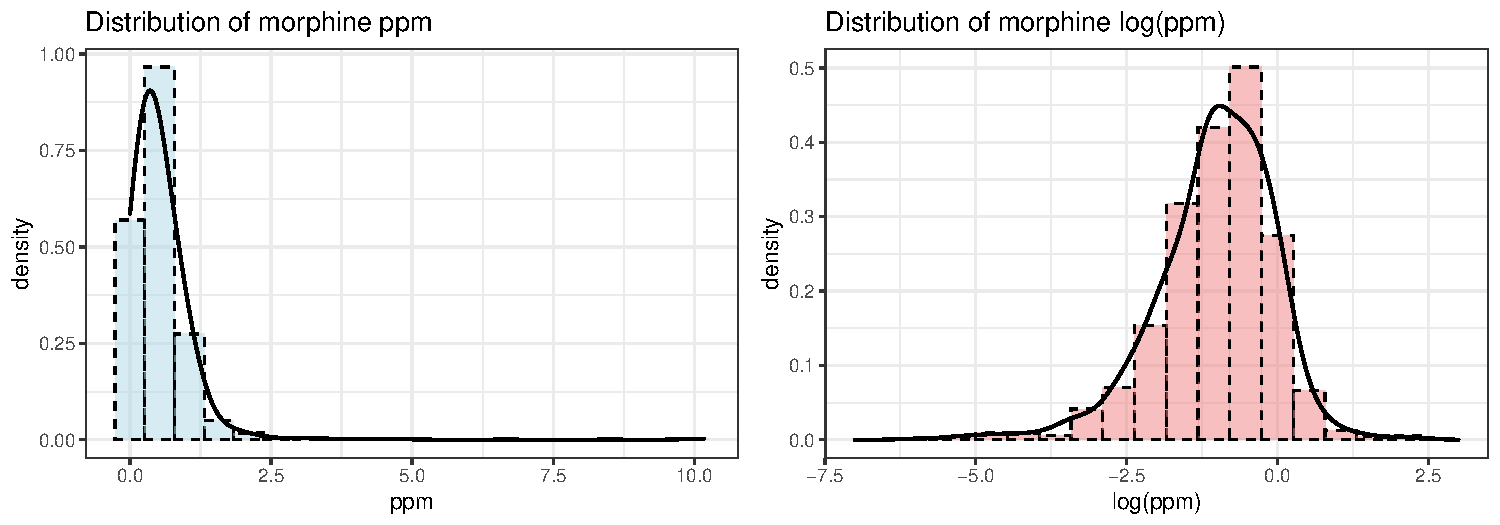
\includegraphics{cs1_files/figure-latex/unnamed-chunk-4-1.pdf}

Whether we fit a hierarchical model or linear regression, the response
variable should be normally distributed. Although the normality
assumption pertains to the conditional distribution of our response
variable, it's still beneficial to check the assumption for the marginal
distribution as a very skewed marginal distribution could persist and
affect the model's resulting conditional distribution. From the
histogram on the left, the distribution of \texttt{ppm} is clearly
right-skewed. Since \texttt{ppm} is strictly non-negative, a log
transformation may be appropriate. We can see that the distribution of
\texttt{log(ppm)}, given above, appears to be much closer to the desired
normal distribution.

\hypertarget{grouping-variable-city-state-and-region}{%
\subsubsection{Grouping Variable: city, state, and
region}\label{grouping-variable-city-state-and-region}}

Since we want to analyze the heterogeneity in pricing by location, we
have three choices of grouping variables, \texttt{city}, \texttt{state},
and \texttt{USA\_region}.

\textbf{City}

There are 1642 unique \texttt{city} values, and many cities have small
sample size (i.e.~less than 5 observations). We decide not to use
\texttt{city} as the grouping variable (see appendix).

\textbf{State}

As for the state, we examined the sample sizes in each group and decided
to filter out Puerto Rico and Vermont because they have less than 5
observations.

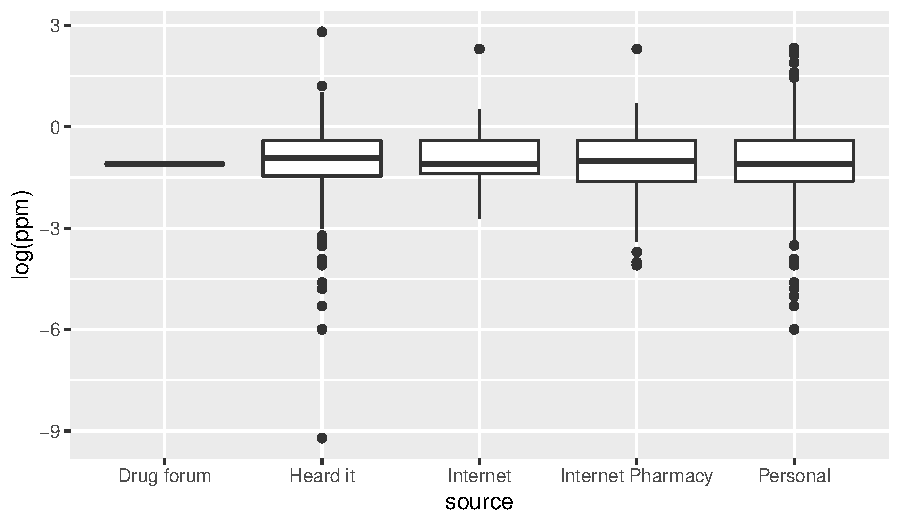
\includegraphics{cs1_files/figure-latex/unnamed-chunk-8-1.pdf}

We then inspect the state-level differences more closely by plotting the
group-level means against the sample sizes. We observed that the
within-state means for states with smaller sample sizes vary a lot,
while the within-state means for states with higher sample sizes in
general adhere more closely to the grand mean. This is conducive to the
borrowing of information between states with a hierarchical model. From
the above boxplot of \texttt{log(ppm)} against \texttt{state}, it is
also evident that the \texttt{log(ppm)} distributions differ across
states. This indicates the potential state-level differences in drug
prices. Therefore, we decide to use state as our grouping variable at
this stage.

\textbf{Region}

From the boxplot we see that the \texttt{log(ppm)} distributions differ
slightly across regions, though not as much as across states. We may
also consider using region as the grouping variable.

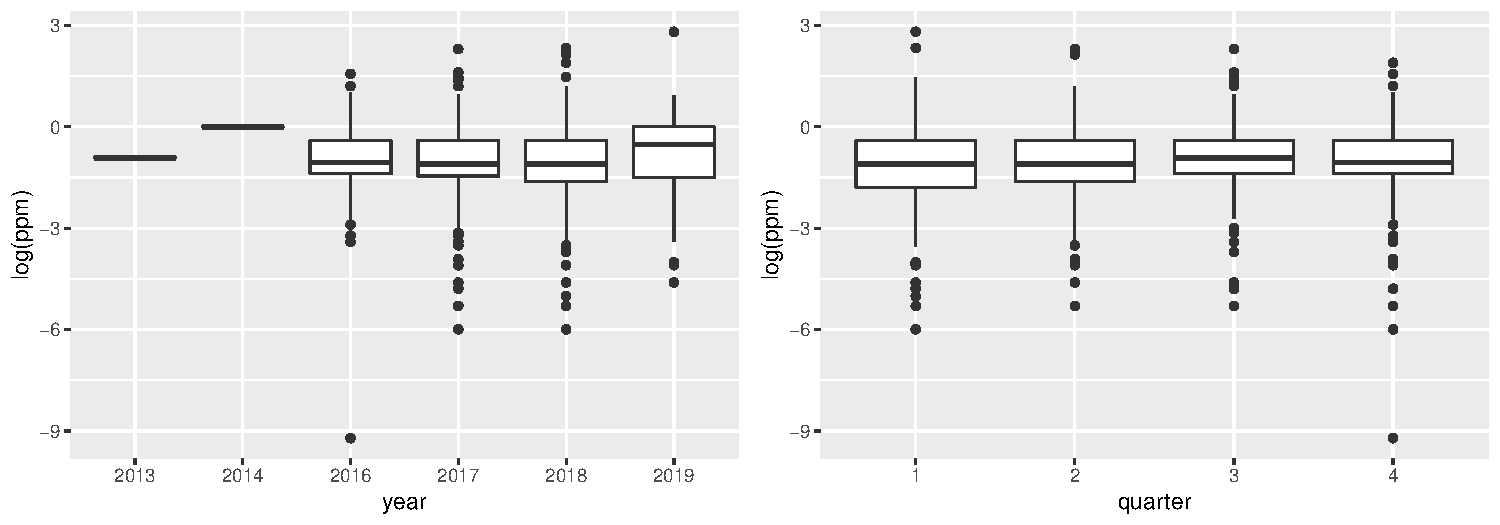
\includegraphics{cs1_files/figure-latex/unnamed-chunk-9-1.pdf}

\hypertarget{date-price_date}{%
\subsubsection{Date (price\_date)}\label{date-price_date}}

As for the \texttt{price\_date}, we noticed some observations are prior
to the establishment of StreetRx, which are likely incorrect inputs. We
dropped the observations before 2010. For the remaining observations, we
came up with two ways of data cleaning. The first choice is to choose a
starting date and convert the feature as the date differences
(\texttt{date\_diff}) from that starting date. The second choice is to
split this date variable into two components, \texttt{year} and
\texttt{quarter}, to explore the trend of unit drug price over time and
the seasonality.

Our visualizations suggested there is no clear indication that the log
value of per milligram price of morphine varies along with
\texttt{date\_diff}. However, for different \texttt{year} and
\texttt{quarter}, the \texttt{log(ppm)} value varies slightly (see
appendix).

\hypertarget{bulk_purchase-source}{%
\subsubsection{Bulk\_purchase \& Source}\label{bulk_purchase-source}}

\includegraphics{cs1_files/figure-latex/unnamed-chunk-16-1.pdf}

There is no need to conduct any data cleaning on
\texttt{bulk\_purchase}. From the boxplot we see that there is a slight
trend that the drug price may be lower if purchased in bulk. Therefore,
\texttt{bulk\_purchase} might be a potential predictor.

For the feature \texttt{source}, we have recoded the missing value as
``Blank'' and the name of websites as ``Internet''. We also dropped the
only observation whose \texttt{source} is ``Drug Forum''. The boxplot
shows that the \texttt{log(ppm)} value varies among different sources
(see appendix).

\hypertarget{dosage-strength-primary-reason}{%
\subsubsection{Dosage Strength \& Primary
Reason}\label{dosage-strength-primary-reason}}

\includegraphics{cs1_files/figure-latex/unnamed-chunk-20-1.pdf}

From the scatter plot of \texttt{log(ppm)} against \texttt{mgstr}, there
is a slight trend that the larger the dosage strength, the smaller the
per milligram price. We have also noticed that \texttt{mgstr} only takes
16 discrete values. Therefore, we decided to transform it into 4 levels
(``low'', ``medium'', ``medium high'', and ``high'') based on the 0.25,
0.5, and 0.75 quantiles of \texttt{mgstr}. From the boxplot, the trend
that the \texttt{log(ppm)} values decrease as the dosage strength
increases is more clear when using these new levels.

For \texttt{primary\_reason}, we have converted the empty cells and ``0
Reporter did not answer this question'' to ``8 Prefer not to answer''.
The \texttt{log(ppm)} value varies among different reasons for
purchasing morphine (see appendix).

\hypertarget{interaction}{%
\subsubsection{Interaction}\label{interaction}}

We also inspected how predictors interact with each other, i.e.~whether
the effect of one predictor on the unit price of morphine is influenced
by any other predictor. We found that there might by potential
interaction among \texttt{dosage\ strength}, and \texttt{quarter}, or
\texttt{quarter}, and \texttt{primary\ reason} (see appendix). In the
modeling part, we will check whether there are interactions in a more
formal way.

\hypertarget{model}{%
\section{Model}\label{model}}

\hypertarget{initial-model-model-selection}{%
\subsubsection{Initial Model \& Model
Selection}\label{initial-model-model-selection}}

The goal of our analysis is to investigate factors related to the per
milligram price of morphine and explore heterogeneity in pricing by
location. As discussed in the EDA part, we do not have enough data to
estimate the effects at the city level. Meanwhile, the drug prices do
not seem to change significantly across regions. Thus, the state
variable is the prefered choice of accounting for location. Since many
states have relatively small sample sizes, a hierarchical model allows
us to borrow information across states.

Comparing three full models with different grouping variables, the AIC
and BIC score also suggest choosing \texttt{state} as the group-level
variable.

\begin{table}

\caption{\label{tab:unnamed-chunk-21}AIC and BIC for different grouping variables}
\centering
\begin{tabular}[t]{l|r|r}
\hline
Grouping & AIC & BIC\\
\hline
City & 15408.58 & 15428.46\\
\hline
State & 15354.88 & 15374.76\\
\hline
Region & 15400.48 & 15420.36\\
\hline
\end{tabular}
\end{table}

Our baseline model incorporates only the state-level random intercepts.
For other individual-level predictors, we add one variable to the model
each time and use both the Likelihood Ratio test and the BIC score to
determine whether it should be added. The LRT is designed for nested
models while the BIC score considers both the likelihood and the model
complexity and gives a more general sense of model performance while
also being consistent. Tables 1 and 2 display the results of model
selection. We also used the full model as a starting point to perform
stepwise backward elimination with the results agreeing with the
previous model selection method. (See appendix).

Our final model incorporates the grouping variable \texttt{state} and
the individual level predictors \texttt{mgstr} (recoded as 4 levels), as
well as \texttt{bulk\_purchase}, \texttt{quarter}, and \texttt{source}.

\begin{table}[!h]

\caption{\label{tab:unnamed-chunk-24}Forward model selection}
\centering
\begin{tabular}[t]{l|l|r}
\hline
Model & LRT.p.value & BIC\\
\hline
\cellcolor{gray!6}{(1|state)} & \cellcolor{gray!6}{} & \cellcolor{gray!6}{15374.76}\\
\hline
(1|state) + mgstr2 & 0 & 14615.63\\
\hline
\cellcolor{gray!6}{(1|state) + mgstr2 + bulk\_purchase} & \cellcolor{gray!6}{2e-04} & \cellcolor{gray!6}{14610.01}\\
\hline
(1|state) + mgstr2 + bulk\_purchase + year & 0.1079 & 14673.21\\
\hline
\cellcolor{gray!6}{(1|state) + mgstr2 + bulk\_purchase + quarter} & \cellcolor{gray!6}{0.0213} & \cellcolor{gray!6}{14626.19}\\
\hline
(1|state) + mgstr2 + bulk\_purchase + date\_diff & 0.1844 & 14616.87\\
\hline
\cellcolor{gray!6}{(1|state) + mgstr2 + bulk\_purchase + quarter + source} & \cellcolor{gray!6}{7e-04} & \cellcolor{gray!6}{14641.45}\\
\hline
(1|state) + mgstr2 + bulk\_purchase + quarter + source + primary\_reason & 1 & 14681.42\\
\hline
\end{tabular}
\end{table}

\hypertarget{interactions}{%
\subsubsection{Interactions}\label{interactions}}

From the EDA, we see some potential interactions between predictors (see
appendix). Here, we also tried to incorporate all possible two-way
interactions into the model (one at a time), but non of them seem to
pass the LRT test or improve the model BIC score (see appendix). To
control the model complexity, we did not try any three-way or more
complex interaction terms. Therefore, we decided not to add any
interaction term into the final model.

\hypertarget{final-model}{%
\subsubsection{Final Model}\label{final-model}}

Our final model is
\[log(y_{ij}) = \beta_0 + b_{0j} + \beta_1 M_{ij} + \beta_2 B_{ij} + \beta_3 Q_{ij} + \beta_4 S_{ij} + \epsilon_{ij}\]
\[b_{0j} \stackrel{iid}\sim \mathcal{N}(0, \tau^2) \perp \epsilon_{ij} \stackrel{iid} \sim \mathcal{N}(0, \sigma^2)\]
The response variable and predictors are defined as:

\begin{itemize}
\item
  \(y_ij\): Per milligram price of morphine for individual i in state j
\item
  \(M_{ij}\): Dosage strength in mg of the units purchased, factored
  into 4 levels
\item
  \(B_{ij}\): Bulk purchase, an indicator for whether 10+ units were
  purchased at once
\item
  \(Q_{ij}\): Quarter of the reported purchase
\item
  \(S_{ij}\): Source of information (including first-hand and
  second-hand sources)
\end{itemize}

\hypertarget{model-diagnostics}{%
\subsubsection{Model Diagnostics}\label{model-diagnostics}}

\includegraphics{cs1_files/figure-latex/unnamed-chunk-28-1.pdf}

\begin{itemize}
\tightlist
\item
  \texttt{Residual\ vs.\ Fitted\ plot}: The residuals are spread equally
  around the horizontal line, indicating there is no non-linear
  relationship.
\item
  \texttt{Normal\ QQ\ plot\ for\ residuals}: The normality assumption is
  slightly met since our residuals adhere around the diagonal line
  representing normality but have heavy tails on both sides. We also
  have one data point that deviates severely from the diagonal line.
\item
  \texttt{Normal\ QQ\ plot\ for\ Random\ Effects}: We can accept the
  random effects are normally distributed. But we still have three
  outliers.
\item
  \texttt{Cook\textquotesingle{}s\ Distance}: We have 3 highly
  influential states (Florida, Pennsylvania, and California) whose
  Cook's distance exceeds the \(\frac{4}{n}\) cutoff, where n denotes
  the number of states.
\end{itemize}

To address the violated assumptions, we tried to remove the data point
with the lowest residual and the influential groups. By removing the
influential observation, the normality of the residuals improved a
little bit, and the dots aligned more tightly to the diagonal line.
However, removing the influential states does not drastically improve
the normality of the residuals (see appendix). Moreover, the influential
states have a considerable sample size (1382 observations). Therefore,
we decide only to drop the individual level outlier but keep all the
groups.

\hypertarget{conclusion}{%
\section{Conclusion}\label{conclusion}}

\hypertarget{fixed-effects}{%
\subsubsection{Fixed Effects}\label{fixed-effects}}

\begin{table}[!h]

\caption{\label{tab:unnamed-chunk-33}Estimates of fixed effects}
\centering
\begin{tabular}[t]{l|r|r|r|r|r|r}
\hline
  & Estimate & exp(Estimate) & Std. Error & df & t value & Pr(>|t|)\\
\hline
\cellcolor{gray!6}{(Intercept)} & \cellcolor{gray!6}{-0.6346} & \cellcolor{gray!6}{0.5301} & \cellcolor{gray!6}{0.0393} & \cellcolor{gray!6}{296.1819} & \cellcolor{gray!6}{-16.1290} & \cellcolor{gray!6}{0.0000}\\
\hline
quarter2 & 0.0854 & 1.0891 & 0.0321 & 5550.5948 & 2.6578 & 0.0079\\
\hline
\cellcolor{gray!6}{quarter3} & \cellcolor{gray!6}{0.0841} & \cellcolor{gray!6}{1.0877} & \cellcolor{gray!6}{0.0332} & \cellcolor{gray!6}{5555.0726} & \cellcolor{gray!6}{2.5349} & \cellcolor{gray!6}{0.0113}\\
\hline
quarter4 & 0.0844 & 1.0881 & 0.0341 & 5551.1650 & 2.4759 & 0.0133\\
\hline
\cellcolor{gray!6}{sourceHeard it} & \cellcolor{gray!6}{0.0633} & \cellcolor{gray!6}{1.0653} & \cellcolor{gray!6}{0.0335} & \cellcolor{gray!6}{5556.1197} & \cellcolor{gray!6}{1.8904} & \cellcolor{gray!6}{0.0588}\\
\hline
sourceInternet & -0.0041 & 0.9959 & 0.0625 & 5555.5822 & -0.0656 & 0.9477\\
\hline
\cellcolor{gray!6}{sourceInternet Pharmacy} & \cellcolor{gray!6}{-0.3227} & \cellcolor{gray!6}{0.7242} & \cellcolor{gray!6}{0.1016} & \cellcolor{gray!6}{5548.9347} & \cellcolor{gray!6}{-3.1743} & \cellcolor{gray!6}{0.0015}\\
\hline
sourcePersonal & -0.0398 & 0.9609 & 0.0281 & 5557.7473 & -1.4157 & 0.1569\\
\hline
\cellcolor{gray!6}{mgstr22 medium} & \cellcolor{gray!6}{-0.3816} & \cellcolor{gray!6}{0.6827} & \cellcolor{gray!6}{0.0279} & \cellcolor{gray!6}{5549.1951} & \cellcolor{gray!6}{-13.6631} & \cellcolor{gray!6}{0.0000}\\
\hline
mgstr23 medium high & -0.7000 & 0.4966 & 0.0365 & 5554.7006 & -19.1836 & 0.0000\\
\hline
\cellcolor{gray!6}{mgstr24 high} & \cellcolor{gray!6}{-1.1197} & \cellcolor{gray!6}{0.3264} & \cellcolor{gray!6}{0.0420} & \cellcolor{gray!6}{5559.7107} & \cellcolor{gray!6}{-26.6889} & \cellcolor{gray!6}{0.0000}\\
\hline
bulk\_purchase1 Bulk purchase & -0.1141 & 0.8922 & 0.0296 & 5557.9880 & -3.8488 & 0.0001\\
\hline
\end{tabular}
\end{table}

\begin{itemize}
\item
  Quarter (baseline: Quarter1): Compared with quarter 1, holding all
  other predictors unchanged, purchasing the morphine in quarter 2, the
  per milligram price of the drug will increase by a multiplicative
  effect of \(e^{0.0853} = 1.0891\) (about 8.91\%). Similarly, if the
  drug is purchased in quarter 3 or 4, the drug price will increase by
  8.77\% and 8.81\%, respectively.
\item
  Source (baseline: Blank): Compared with an unknown source, holding all
  other predictors unchanged, the per milligram drug price heard from
  other people will increase by a multiplicative effect of
  \(e^{0.0633} = 1.0653\) (about 6.53\%). Similarly, the price
  information obtained from the internet, internet pharmacy, or personal
  purchase will decrease by 0.41\%, 27.58\%, and 3.91\%, respectively.
\item
  Dosage Strength (baseline: Low): Compared with low dosage strength,
  holding all other predictors unchanged, the per milligram price of
  morphine will decrease by a multiplicative effect of
  \(e^{-0.3816} = 0.6827\) (about 31.73\%) if it has medium dosage
  strength. Similarly, if the dosage strength is medium-high or high,
  the drug price will decrease by 50.34\% and 67.36\%, respectively.
\item
  Bulk Purchase (baseline: Not bulk purchase): Compared with non-bulk
  purchase, holding all other predictors unchanged, the unit price of
  morphine will decrease by a multiplicative effect of
  \(e^{0.1141} = 0.8922\) (about 10.78\%).
\end{itemize}

\hypertarget{random-effects}{%
\subsubsection{Random Effects}\label{random-effects}}

\begin{table}[!h]

\caption{\label{tab:unnamed-chunk-34}Estimates of random effects}
\centering
\begin{tabular}[t]{l|r|r}
\hline
  & $\tau^2$ & $\sigma^2$\\
\hline
\cellcolor{gray!6}{Estimate} & \cellcolor{gray!6}{0.0161} & \cellcolor{gray!6}{0.7772}\\
\hline
\end{tabular}
\end{table}

The estimated across-state variance is \(\hat{\tau^2} = 0.0161\), which
also describes the variation attributed to the random intercept. The
estimated within-state variance is \(\hat{\sigma^2} = 0.7772\), which
describes the unexplained variation. The estimated interclass
correlation is
\(\frac{\hat{\tau^2}}{\hat{\tau^2} + \hat{\sigma^2}} \approx 0.02\).
Therefore, we have little correlation within the same state.

\includegraphics{cs1_files/figure-latex/unnamed-chunk-35-1.pdf}

From the random intercepts plot, we can see that states have different
bases per milligram morphine prices. The prices ranges from
\(e^{-0.2297} = 0.7948\) (Michigan) to \(e^{0.2063} = 1.2292\)
(Massachusetts). These estimates are based on the baseline condition of
all other predictors, which are purchasing in quarter 1, from an unknown
source, with low dosage strength, and not purchased in bulk

\hypertarget{limitations}{%
\section{Limitations}\label{limitations}}

Our analysis and model have several limitations. Firstly, StreetRX
provides only self-reported data, which is likely to be messy, biased,
and lacking credibility. Although we borrow information across states
via a hierarchical model, states with small sample sizes are still
problematic. The within-state variance \(\sigma^2\) is much larger than
the across-state variance \(\tau^2\), indicating that there is still
much within-state variation left unexplained. This suggests that the per
milligram price of morphine may depend on factors not on the state
level. Having access to more predictors may help explain these
variations and improve the model performance.

Another line

Another line 2

\newpage

\hypertarget{appendix}{%
\section{Appendix}\label{appendix}}

\hypertarget{additional-tables-and-figures}{%
\subsection{Additional tables and
figures}\label{additional-tables-and-figures}}

\hypertarget{data-cleaning-eda-1}{%
\subsubsection{Data Cleaning \& EDA}\label{data-cleaning-eda-1}}

\hypertarget{missing-values-1}{%
\subsubsection{Missing Values}\label{missing-values-1}}

\begin{center}\includegraphics{cs1_files/figure-latex/unnamed-chunk-38-1} \end{center}

\hypertarget{grouping-variable-city-state-and-region-1}{%
\subsubsection{Grouping Variable: city, state, and
region}\label{grouping-variable-city-state-and-region-1}}

\textbf{State}

\hypertarget{date-price_date-1}{%
\subsubsection{Date (price\_date)}\label{date-price_date-1}}

\begin{center}\includegraphics{cs1_files/figure-latex/unnamed-chunk-45-1} \end{center}

\begin{center}\includegraphics{cs1_files/figure-latex/unnamed-chunk-46-1} \end{center}

\hypertarget{dosage-strength-primary-reason-1}{%
\subsubsection{Dosage Strength \& Primary
Reason}\label{dosage-strength-primary-reason-1}}

\begin{center}\includegraphics{cs1_files/figure-latex/unnamed-chunk-47-1} \end{center}

\begin{table}

\caption{\label{tab:unnamed-chunk-49}Quantile of mgstr}
\centering
\begin{tabular}[t]{l|r}
\hline
  & mgstr\\
\hline
25\% & 15\\
\hline
50\% & 30\\
\hline
75\% & 60\\
\hline
\end{tabular}
\end{table}

\hypertarget{interaction-plots}{%
\subsubsection{Interaction Plots}\label{interaction-plots}}

\begin{center}\includegraphics{cs1_files/figure-latex/unnamed-chunk-51-1} \end{center}

\begin{center}\includegraphics{cs1_files/figure-latex/unnamed-chunk-51-2} \end{center}

\begin{center}\includegraphics{cs1_files/figure-latex/unnamed-chunk-51-3} \end{center}

\begin{center}\includegraphics{cs1_files/figure-latex/unnamed-chunk-51-4} \end{center}

\hypertarget{model-1}{%
\subsection{Model}\label{model-1}}

\hypertarget{initial-model-model-selection-1}{%
\subsubsection{Initial Model \& Model
Selection}\label{initial-model-model-selection-1}}

\begin{table}[!h]

\caption{\label{tab:unnamed-chunk-52}AIC and BIC for different grouping variables (full models)}
\centering
\begin{tabular}[t]{l|r|r}
\hline
Grouping & AIC & BIC\\
\hline
\cellcolor{gray!6}{City} & \cellcolor{gray!6}{14627.21} & \cellcolor{gray!6}{14931.96}\\
\hline
State & 14577.10 & 14881.85\\
\hline
\cellcolor{gray!6}{Region} & \cellcolor{gray!6}{14610.16} & \cellcolor{gray!6}{14914.91}\\
\hline
\end{tabular}
\end{table}

\begin{table}

\caption{\label{tab:unnamed-chunk-53}Stepwise backward elimination results}
\centering
\begin{tabular}[t]{l|r|r|r|r|r|r|r}
\hline
  & Eliminated & Sum Sq & Mean Sq & NumDF & DenDF & F value & Pr(>F)\\
\hline
date\_diff & 1 & 0.0173 & 0.0173 & 1 & 5560.078 & 0.0221 & 0.8817\\
\hline
year & 2 & 8.1386 & 0.9043 & 9 & 5549.587 & 1.1558 & 0.3191\\
\hline
primary\_reason & 3 & 11.3847 & 1.4231 & 8 & 5552.196 & 1.8156 & 0.0693\\
\hline
quarter & 0 & 7.1468 & 2.3823 & 3 & 5554.311 & 3.0310 & 0.0282\\
\hline
mgstr2 & 0 & 670.1758 & 223.3919 & 3 & 5554.045 & 284.2265 & 0.0000\\
\hline
bulk\_purchase & 0 & 12.1690 & 12.1690 & 1 & 5560.929 & 15.4829 & 0.0001\\
\hline
source & 0 & 24.8908 & 1.3828 & 18 & 5550.635 & 1.7594 & 0.0243\\
\hline
\end{tabular}
\end{table}

\hypertarget{interactions-1}{%
\subsubsection{Interactions}\label{interactions-1}}

\begin{table}[!h]

\caption{\label{tab:unnamed-chunk-54}Interaction}
\centering
\begin{tabular}[t]{l|l|r}
\hline
Model & LRT.p.value & BIC\\
\hline
\cellcolor{gray!6}{without interaction} & \cellcolor{gray!6}{} & \cellcolor{gray!6}{14751.51}\\
\hline
+ quarter x bulk\_purchase & 0.1566 & 14772.17\\
\hline
\cellcolor{gray!6}{+ quarter x mgstr2} & \cellcolor{gray!6}{0.4914} & \cellcolor{gray!6}{14820.71}\\
\hline
+ bulk\_purchase x mgstr2 & 0.1411 & 14771.93\\
\hline
\cellcolor{gray!6}{+ quarter x source} & \cellcolor{gray!6}{0.0022} & \cellcolor{gray!6}{14831.35}\\
\hline
+ bulk\_purchase x source & 0.5854 & 14783.18\\
\hline
\cellcolor{gray!6}{+ source x mgstr2} & \cellcolor{gray!6}{0.9947} & \cellcolor{gray!6}{14948.55}\\
\hline
\end{tabular}
\end{table}

\hypertarget{model-diagnostics-1}{%
\subsubsection{Model Diagnostics}\label{model-diagnostics-1}}

\textbf{Diagnostic plots for model\_g2 (drop one observation with the
lowest residual in model\_g)}

\textbf{Diagnostic plots for model\_g3 (drop influential states)}

\begin{center}\includegraphics{cs1_files/figure-latex/unnamed-chunk-58-1} \end{center}

\hypertarget{conclusion-1}{%
\subsection{Conclusion}\label{conclusion-1}}

\hypertarget{fixed-effects-1}{%
\subsubsection{Fixed Effects}\label{fixed-effects-1}}

\begin{table}[!h]

\caption{\label{tab:unnamed-chunk-60}Estimates of fixed effects}
\centering
\begin{tabular}[t]{l|r|r|r|r|r|r}
\hline
  & Estimate & exp(Estimate) & Std. Error & df & t value & Pr(>|t|)\\
\hline
\cellcolor{gray!6}{(Intercept)} & \cellcolor{gray!6}{-0.6346} & \cellcolor{gray!6}{0.5301} & \cellcolor{gray!6}{0.0393} & \cellcolor{gray!6}{296.1819} & \cellcolor{gray!6}{-16.1290} & \cellcolor{gray!6}{0.0000}\\
\hline
quarter2 & 0.0854 & 1.0891 & 0.0321 & 5550.5948 & 2.6578 & 0.0079\\
\hline
\cellcolor{gray!6}{quarter3} & \cellcolor{gray!6}{0.0841} & \cellcolor{gray!6}{1.0877} & \cellcolor{gray!6}{0.0332} & \cellcolor{gray!6}{5555.0726} & \cellcolor{gray!6}{2.5349} & \cellcolor{gray!6}{0.0113}\\
\hline
quarter4 & 0.0844 & 1.0881 & 0.0341 & 5551.1650 & 2.4759 & 0.0133\\
\hline
\cellcolor{gray!6}{sourceHeard it} & \cellcolor{gray!6}{0.0633} & \cellcolor{gray!6}{1.0653} & \cellcolor{gray!6}{0.0335} & \cellcolor{gray!6}{5556.1197} & \cellcolor{gray!6}{1.8904} & \cellcolor{gray!6}{0.0588}\\
\hline
sourceInternet & -0.0041 & 0.9959 & 0.0625 & 5555.5822 & -0.0656 & 0.9477\\
\hline
\cellcolor{gray!6}{sourceInternet Pharmacy} & \cellcolor{gray!6}{-0.3227} & \cellcolor{gray!6}{0.7242} & \cellcolor{gray!6}{0.1016} & \cellcolor{gray!6}{5548.9347} & \cellcolor{gray!6}{-3.1743} & \cellcolor{gray!6}{0.0015}\\
\hline
sourcePersonal & -0.0398 & 0.9609 & 0.0281 & 5557.7473 & -1.4157 & 0.1569\\
\hline
\cellcolor{gray!6}{mgstr22 medium} & \cellcolor{gray!6}{-0.3816} & \cellcolor{gray!6}{0.6827} & \cellcolor{gray!6}{0.0279} & \cellcolor{gray!6}{5549.1951} & \cellcolor{gray!6}{-13.6631} & \cellcolor{gray!6}{0.0000}\\
\hline
mgstr23 medium high & -0.7000 & 0.4966 & 0.0365 & 5554.7006 & -19.1836 & 0.0000\\
\hline
\cellcolor{gray!6}{mgstr24 high} & \cellcolor{gray!6}{-1.1197} & \cellcolor{gray!6}{0.3264} & \cellcolor{gray!6}{0.0420} & \cellcolor{gray!6}{5559.7107} & \cellcolor{gray!6}{-26.6889} & \cellcolor{gray!6}{0.0000}\\
\hline
bulk\_purchase1 Bulk purchase & -0.1141 & 0.8922 & 0.0296 & 5557.9880 & -3.8488 & 0.0001\\
\hline
\end{tabular}
\end{table}

\hypertarget{random-effects-1}{%
\subsubsection{Random Effects}\label{random-effects-1}}

\begin{longtable}[t]{l|l|l|r|r|r}
\caption{\label{tab:unnamed-chunk-61}Estimated random intercepts}\\
\hline
grpvar & term & grp & condval & condsd & exp(condval)\\
\hline
state & (Intercept) & Massachusetts & 0.2063 & 0.0761 & 1.2292\\
\hline
state & (Intercept) & New Jersey & 0.1713 & 0.0784 & 1.1869\\
\hline
state & (Intercept) & Tennessee & 0.1702 & 0.0611 & 1.1855\\
\hline
state & (Intercept) & Maine & 0.1189 & 0.1091 & 1.1263\\
\hline
state & (Intercept) & Virginia & 0.1144 & 0.0766 & 1.1212\\
\hline
state & (Intercept) & Mississippi & 0.1130 & 0.0984 & 1.1197\\
\hline
state & (Intercept) & Louisiana & 0.1127 & 0.0851 & 1.1193\\
\hline
state & (Intercept) & Maryland & 0.0953 & 0.0784 & 1.1000\\
\hline
state & (Intercept) & West Virginia & 0.0774 & 0.1037 & 1.0805\\
\hline
state & (Intercept) & Alaska & 0.0762 & 0.1145 & 1.0792\\
\hline
state & (Intercept) & Kansas & 0.0739 & 0.0898 & 1.0767\\
\hline
state & (Intercept) & Kentucky & 0.0716 & 0.0843 & 1.0743\\
\hline
state & (Intercept) & Oklahoma & 0.0712 & 0.0631 & 1.0738\\
\hline
state & (Intercept) & New Hampshire & 0.0697 & 0.1154 & 1.0721\\
\hline
state & (Intercept) & Arkansas & 0.0558 & 0.0804 & 1.0573\\
\hline
state & (Intercept) & Washington, DC & 0.0546 & 0.1154 & 1.0561\\
\hline
state & (Intercept) & Utah & 0.0244 & 0.0908 & 1.0247\\
\hline
state & (Intercept) & Nebraska & 0.0221 & 0.0966 & 1.0224\\
\hline
state & (Intercept) & Alabama & 0.0181 & 0.0682 & 1.0182\\
\hline
state & (Intercept) & Montana & 0.0152 & 0.1083 & 1.0153\\
\hline
state & (Intercept) & South Dakota & 0.0152 & 0.1185 & 1.0153\\
\hline
state & (Intercept) & Wisconsin & 0.0120 & 0.0726 & 1.0121\\
\hline
state & (Intercept) & Iowa & 0.0096 & 0.0839 & 1.0097\\
\hline
state & (Intercept) & Rhode Island & 0.0074 & 0.1117 & 1.0074\\
\hline
state & (Intercept) & Wyoming & 0.0021 & 0.1175 & 1.0021\\
\hline
state & (Intercept) & Florida & -0.0049 & 0.0415 & 0.9951\\
\hline
state & (Intercept) & Minnesota & -0.0054 & 0.0867 & 0.9946\\
\hline
state & (Intercept) & Indiana & -0.0109 & 0.0655 & 0.9891\\
\hline
state & (Intercept) & Washington & -0.0119 & 0.0550 & 0.9881\\
\hline
state & (Intercept) & North Dakota & -0.0139 & 0.1207 & 0.9862\\
\hline
state & (Intercept) & Missouri & -0.0150 & 0.0657 & 0.9851\\
\hline
state & (Intercept) & Colorado & -0.0157 & 0.0677 & 0.9844\\
\hline
state & (Intercept) & Oregon & -0.0181 & 0.0615 & 0.9820\\
\hline
state & (Intercept) & Pennsylvania & -0.0185 & 0.0523 & 0.9816\\
\hline
state & (Intercept) & Idaho & -0.0188 & 0.1051 & 0.9814\\
\hline
state & (Intercept) & Texas & -0.0342 & 0.0448 & 0.9663\\
\hline
state & (Intercept) & New York & -0.0385 & 0.0564 & 0.9623\\
\hline
state & (Intercept) & Ohio & -0.0412 & 0.0573 & 0.9596\\
\hline
state & (Intercept) & North Carolina & -0.0444 & 0.0668 & 0.9565\\
\hline
state & (Intercept) & Delaware & -0.0548 & 0.1108 & 0.9466\\
\hline
state & (Intercept) & New Mexico & -0.0792 & 0.0984 & 0.9239\\
\hline
state & (Intercept) & Illinois & -0.0917 & 0.0666 & 0.9124\\
\hline
state & (Intercept) & Hawaii & -0.0944 & 0.1009 & 0.9100\\
\hline
state & (Intercept) & Nevada & -0.1057 & 0.0664 & 0.8997\\
\hline
state & (Intercept) & Georgia & -0.1287 & 0.0629 & 0.8793\\
\hline
state & (Intercept) & Connecticut & -0.1363 & 0.0960 & 0.8726\\
\hline
state & (Intercept) & South Carolina & -0.1379 & 0.0775 & 0.8712\\
\hline
state & (Intercept) & California & -0.2098 & 0.0313 & 0.8107\\
\hline
state & (Intercept) & Arizona & -0.2192 & 0.0514 & 0.8031\\
\hline
state & (Intercept) & Michigan & -0.2297 & 0.0490 & 0.7948\\
\hline
\end{longtable}
\newpage

\hypertarget{codes}{%
\subsection{Codes}\label{codes}}

\begin{Shaded}
\begin{Highlighting}[]
\NormalTok{knitr}\OperatorTok{::}\NormalTok{opts_chunk}\OperatorTok{$}\KeywordTok{set}\NormalTok{(}\DataTypeTok{warning=}\OtherTok{FALSE}\NormalTok{, }\DataTypeTok{message =} \OtherTok{FALSE}\NormalTok{, }\DataTypeTok{cache =} \OtherTok{TRUE}\NormalTok{)}
\KeywordTok{library}\NormalTok{(tidyverse)}
\KeywordTok{library}\NormalTok{(janitor)}
\KeywordTok{library}\NormalTok{(gridExtra)}
\KeywordTok{library}\NormalTok{(cowplot)}
\KeywordTok{library}\NormalTok{(knitr)}
\KeywordTok{require}\NormalTok{(magrittr)}
\KeywordTok{require}\NormalTok{(dplyr)}
\KeywordTok{library}\NormalTok{(kableExtra)}
\KeywordTok{library}\NormalTok{(readr)}
\KeywordTok{library}\NormalTok{(tidyr)}
\KeywordTok{library}\NormalTok{(broom)}
\KeywordTok{library}\NormalTok{(lme4)}
\KeywordTok{library}\NormalTok{(glmmTMB)}
\KeywordTok{library}\NormalTok{(sjPlot)}
\KeywordTok{library}\NormalTok{(brms)}
\KeywordTok{library}\NormalTok{(coda)}
\KeywordTok{library}\NormalTok{(rstan)}
\KeywordTok{library}\NormalTok{(tidybayes)}
\KeywordTok{library}\NormalTok{(naniar)}
\KeywordTok{library}\NormalTok{(olsrr)}
\KeywordTok{library}\NormalTok{(lmerTest)}
\KeywordTok{require}\NormalTok{(lattice)}

\CommentTok{# devtools::install_github("goodekat/redres")}
\CommentTok{#library(redres)}
\end{Highlighting}
\end{Shaded}

\begin{Shaded}
\begin{Highlighting}[]
\KeywordTok{load}\NormalTok{(}\StringTok{'streetrx.RData'}\NormalTok{)}
\end{Highlighting}
\end{Shaded}

\begin{Shaded}
\begin{Highlighting}[]
\NormalTok{na_check <-}\StringTok{ }\NormalTok{streetrx }\OperatorTok
\StringTok{  }\KeywordTok{filter}\NormalTok{(api_temp }\OperatorTok{==}\StringTok{ 'morphine'}\NormalTok{) }\OperatorTok
\StringTok{  }\KeywordTok{mutate_all}\NormalTok{( }\KeywordTok{list}\NormalTok{( }\OperatorTok{~}\KeywordTok{na_if}\NormalTok{(., }\StringTok{''}\NormalTok{) ) ) }\OperatorTok
\StringTok{  }\KeywordTok{droplevels}\NormalTok{()}

\KeywordTok{dim}\NormalTok{(na_check)}
\KeywordTok{sum}\NormalTok{(}\KeywordTok{is.na}\NormalTok{(na_check))}

\KeywordTok{sum}\NormalTok{(}\KeywordTok{is.na}\NormalTok{(na_check}\OperatorTok{$}\NormalTok{Primary_Reason))}

\KeywordTok{sum}\NormalTok{(}\KeywordTok{is.na}\NormalTok{(na_check}\OperatorTok{$}\NormalTok{source))}

\KeywordTok{sum}\NormalTok{(}\KeywordTok{is.na}\NormalTok{(na_check))}

\KeywordTok{gg_miss_upset}\NormalTok{(na_check)}
\end{Highlighting}
\end{Shaded}

\begin{Shaded}
\begin{Highlighting}[]
\CommentTok{# subset for group drug}

\NormalTok{morph_data <-}\StringTok{ }\NormalTok{streetrx }\OperatorTok
\StringTok{  }\KeywordTok{filter}\NormalTok{(api_temp }\OperatorTok{==}\StringTok{ 'morphine'}\NormalTok{)}

\NormalTok{morph_data}\OperatorTok{$}\NormalTok{Primary_Reason <-}\StringTok{ }\KeywordTok{droplevels}\NormalTok{(morph_data}\OperatorTok{$}\NormalTok{Primary_Reason)}
\KeywordTok{levels}\NormalTok{(morph_data}\OperatorTok{$}\NormalTok{Primary_Reason)[}\DecValTok{1}\NormalTok{] <-}\StringTok{ "8 Prefer not to answer"}
\KeywordTok{levels}\NormalTok{(morph_data}\OperatorTok{$}\NormalTok{Primary_Reason)[}\DecValTok{2}\NormalTok{] <-}\StringTok{ "8 Prefer not to answer"}

\NormalTok{morph_data}\OperatorTok{$}\NormalTok{source <-}\StringTok{ }\KeywordTok{droplevels}\NormalTok{(morph_data}\OperatorTok{$}\NormalTok{source)}
\KeywordTok{levels}\NormalTok{(morph_data}\OperatorTok{$}\NormalTok{source)[}\DecValTok{1}\NormalTok{] <-}\StringTok{ "Blank"}

\NormalTok{morph_data <-}\StringTok{ }\NormalTok{morph_data }\OperatorTok\StringTok{ }
\StringTok{  }\KeywordTok{filter}\NormalTok{(}\KeywordTok{between}\NormalTok{(ppm, }\FloatTok{0.000001}\NormalTok{, }\DecValTok{10}\NormalTok{)) }\OperatorTok
\StringTok{  }\KeywordTok{mutate_all}\NormalTok{( }\KeywordTok{list}\NormalTok{( }\OperatorTok{~}\KeywordTok{na_if}\NormalTok{(., }\StringTok{''}\NormalTok{) ) ) }\OperatorTok
\StringTok{  }\KeywordTok{drop_na}\NormalTok{() }\OperatorTok
\StringTok{  }\KeywordTok{clean_names}\NormalTok{() }\OperatorTok
\StringTok{  }\KeywordTok{mutate}\NormalTok{(}
    \DataTypeTok{quarter=}\KeywordTok{substring}\NormalTok{(yq_pdate, }\DecValTok{5}\NormalTok{, }\DecValTok{5}\NormalTok{),}
    \DataTypeTok{year=}\KeywordTok{substring}\NormalTok{(yq_pdate, }\DecValTok{1}\NormalTok{, }\DecValTok{4}\NormalTok{),}
    \DataTypeTok{state=}\KeywordTok{recode_factor}\NormalTok{(}\KeywordTok{droplevels}\NormalTok{(state), }\StringTok{'USA'}\NormalTok{=}\StringTok{'Unknown'}\NormalTok{)}
\NormalTok{  ) }

\KeywordTok{nrow}\NormalTok{(morph_data)}

\KeywordTok{sum}\NormalTok{(morph_data}\OperatorTok{$}\NormalTok{ppm }\OperatorTok{<=}\DecValTok{0}\NormalTok{)}
\end{Highlighting}
\end{Shaded}

\begin{Shaded}
\begin{Highlighting}[]
\CommentTok{# remove extreme outliers based on quantiles}

\CommentTok{# untransformed density}
\NormalTok{p1 <-}\StringTok{ }\NormalTok{morph_data }\OperatorTok
\StringTok{  }\KeywordTok{ggplot}\NormalTok{(}\KeywordTok{aes}\NormalTok{(}\DataTypeTok{x=}\NormalTok{ppm)) }\OperatorTok{+}
\StringTok{    }\KeywordTok{geom_histogram}\NormalTok{(}
      \KeywordTok{aes}\NormalTok{(}\DataTypeTok{y=}\NormalTok{..density..), }
      \DataTypeTok{color=}\StringTok{'black'}\NormalTok{, }
      \DataTypeTok{linetype=}\StringTok{'dashed'}\NormalTok{,}
      \DataTypeTok{size=}\FloatTok{0.5}\NormalTok{,}
      \DataTypeTok{fill=}\StringTok{'lightblue'}\NormalTok{, }
      \DataTypeTok{alpha=}\FloatTok{0.5}\NormalTok{,}
      \DataTypeTok{bins=}\DecValTok{20}
\NormalTok{    ) }\OperatorTok{+}
\StringTok{    }\KeywordTok{geom_density}\NormalTok{(}\DataTypeTok{size=}\FloatTok{0.75}\NormalTok{, }\DataTypeTok{bw=}\FloatTok{0.3}\NormalTok{) }\OperatorTok{+}
\StringTok{    }\KeywordTok{ggtitle}\NormalTok{(}\StringTok{"Figure 1: Distribution of morphine ppm"}\NormalTok{) }\OperatorTok{+}
\StringTok{    }\KeywordTok{theme}\NormalTok{(}\DataTypeTok{plot.title =} \KeywordTok{element_text}\NormalTok{(}\DataTypeTok{hjust =} \FloatTok{0.5}\NormalTok{))}



\CommentTok{# log-transformed density}
\NormalTok{p2 <-}\StringTok{ }\NormalTok{morph_data }\OperatorTok
\StringTok{  }\KeywordTok{ggplot}\NormalTok{(}\KeywordTok{aes}\NormalTok{(}\DataTypeTok{x=}\KeywordTok{log}\NormalTok{(ppm))) }\OperatorTok{+}
\StringTok{    }\KeywordTok{geom_histogram}\NormalTok{(}
      \KeywordTok{aes}\NormalTok{(}\DataTypeTok{y=}\NormalTok{..density..), }
      \DataTypeTok{color=}\StringTok{'black'}\NormalTok{, }
      \DataTypeTok{linetype=}\StringTok{'dashed'}\NormalTok{,}
      \DataTypeTok{size=}\FloatTok{0.5}\NormalTok{,}
      \DataTypeTok{fill=}\StringTok{'lightcoral'}\NormalTok{, }
      \DataTypeTok{alpha=}\FloatTok{0.5}\NormalTok{,}
      \DataTypeTok{bins=}\DecValTok{20}
\NormalTok{    ) }\OperatorTok{+}
\StringTok{    }\KeywordTok{geom_density}\NormalTok{(}\DataTypeTok{size=}\FloatTok{0.75}\NormalTok{, }\DataTypeTok{bw=}\FloatTok{0.3}\NormalTok{) }\OperatorTok{+}
\StringTok{    }\KeywordTok{xlim}\NormalTok{(}\OperatorTok{-}\DecValTok{7}\NormalTok{, }\DecValTok{3}\NormalTok{) }\OperatorTok{+}
\StringTok{    }\KeywordTok{ggtitle}\NormalTok{(}\StringTok{"Figure 2: Distribution of morphine log(ppm)"}\NormalTok{) }\OperatorTok{+}
\StringTok{    }\KeywordTok{theme}\NormalTok{(}\DataTypeTok{plot.title =} \KeywordTok{element_text}\NormalTok{(}\DataTypeTok{hjust =} \FloatTok{0.5}\NormalTok{))}

\KeywordTok{grid.arrange}\NormalTok{(p1, p2, }\DataTypeTok{ncol=}\DecValTok{2}\NormalTok{)}
\end{Highlighting}
\end{Shaded}

\begin{Shaded}
\begin{Highlighting}[]
\KeywordTok{length}\NormalTok{(}\KeywordTok{unique}\NormalTok{(morph_data}\OperatorTok{$}\NormalTok{city))}
\KeywordTok{length}\NormalTok{(}\KeywordTok{unique}\NormalTok{(morph_data}\OperatorTok{$}\NormalTok{state))}
\KeywordTok{length}\NormalTok{(}\KeywordTok{unique}\NormalTok{(morph_data}\OperatorTok{$}\NormalTok{usa_region))}
\end{Highlighting}
\end{Shaded}

\begin{Shaded}
\begin{Highlighting}[]
\NormalTok{state_size <-}\StringTok{ }\NormalTok{morph_data }\OperatorTok
\StringTok{  }\KeywordTok{group_by}\NormalTok{(state) }\OperatorTok
\StringTok{  }\KeywordTok{summarise}\NormalTok{(}\DataTypeTok{n =} \KeywordTok{n}\NormalTok{(), }\DataTypeTok{.groups =} \StringTok{"drop"}\NormalTok{)  }\OperatorTok
\StringTok{  }\KeywordTok{arrange}\NormalTok{(n) }\OperatorTok
\StringTok{  }\KeywordTok{pivot_wider}\NormalTok{(}
    \DataTypeTok{names_from=}\NormalTok{state,}
    \DataTypeTok{values_from=}\NormalTok{n}
\NormalTok{  )}

\NormalTok{state_size }\OperatorTok\StringTok{ }
\StringTok{  }\NormalTok{dplyr}\OperatorTok{::}\KeywordTok{select}\NormalTok{(}\DecValTok{1}\OperatorTok{:}\DecValTok{5}\NormalTok{) }\OperatorTok
\StringTok{  }\KeywordTok{kable}\NormalTok{(}
    \DataTypeTok{caption =} \StringTok{'5 States with Smallest Sample Size'}\NormalTok{,}
    \DataTypeTok{align=}\StringTok{'c'}\NormalTok{, }
    \DataTypeTok{booktabs=}\OtherTok{TRUE}\NormalTok{) }\OperatorTok
\StringTok{  }\KeywordTok{kable_styling}\NormalTok{(}\DataTypeTok{latex_options =} \KeywordTok{c}\NormalTok{(}\StringTok{'hold_position'}\NormalTok{))}
\end{Highlighting}
\end{Shaded}

\begin{Shaded}
\begin{Highlighting}[]
\CommentTok{# remove low sample size states}
\NormalTok{morph_data <-}\StringTok{ }\NormalTok{morph_data }\OperatorTok
\StringTok{  }\KeywordTok{mutate}\NormalTok{(}\DataTypeTok{state=}\KeywordTok{as.character}\NormalTok{(state)) }\OperatorTok
\StringTok{  }\KeywordTok{filter}\NormalTok{(}\OperatorTok{!}\NormalTok{state }\OperatorTok\StringTok{ }\KeywordTok{c}\NormalTok{(}
    \StringTok{'Puerto Rico'}\NormalTok{, }\StringTok{'Vermont'}
\NormalTok{  ))}
\end{Highlighting}
\end{Shaded}

\begin{Shaded}
\begin{Highlighting}[]
\NormalTok{morph_state <-}\StringTok{ }\NormalTok{morph_data }\OperatorTok
\StringTok{  }\KeywordTok{filter}\NormalTok{(state }\OperatorTok\StringTok{ }\NormalTok{state.name) }\OperatorTok
\StringTok{  }\KeywordTok{mutate}\NormalTok{(}\DataTypeTok{state_abv=}\NormalTok{state.abb[}\KeywordTok{match}\NormalTok{(state,state.name)])}


\NormalTok{grand_mean <-}\StringTok{ }\KeywordTok{mean}\NormalTok{(morph_state}\OperatorTok{$}\NormalTok{ppm)}

\NormalTok{p3 <-}\StringTok{ }\NormalTok{morph_state }\OperatorTok
\StringTok{  }\KeywordTok{group_by}\NormalTok{(state_abv) }\OperatorTok
\StringTok{  }\KeywordTok{summarise}\NormalTok{(}\DataTypeTok{n =} \KeywordTok{n}\NormalTok{(), }\DataTypeTok{mean =} \KeywordTok{mean}\NormalTok{(ppm)) }\OperatorTok
\StringTok{  }\KeywordTok{ggplot}\NormalTok{(}\KeywordTok{aes}\NormalTok{(}\DataTypeTok{x=}\NormalTok{n, }\DataTypeTok{y=}\NormalTok{mean)) }\OperatorTok{+}
\StringTok{    }\KeywordTok{geom_hline}\NormalTok{(}
      \KeywordTok{aes}\NormalTok{(}\DataTypeTok{yintercept=}\NormalTok{grand_mean),}
      \DataTypeTok{linetype=}\StringTok{'dashed'}\NormalTok{,}
      \DataTypeTok{color=}\StringTok{'red'}\NormalTok{,}
      \DataTypeTok{size=}\FloatTok{0.75}
\NormalTok{    ) }\OperatorTok{+}
\StringTok{    }\KeywordTok{geom_point}\NormalTok{() }\OperatorTok{+}
\StringTok{    }\KeywordTok{labs}\NormalTok{(}\DataTypeTok{x=}\StringTok{'sample size'}\NormalTok{, }\DataTypeTok{y=}\StringTok{'mean log(ppm)'}\NormalTok{) }\OperatorTok{+}
\StringTok{    }\KeywordTok{ggtitle}\NormalTok{(}\StringTok{"Figure 3: Group mean vs. sample size"}\NormalTok{) }\OperatorTok{+}
\StringTok{    }\KeywordTok{theme}\NormalTok{(}\DataTypeTok{plot.title =} \KeywordTok{element_text}\NormalTok{(}\DataTypeTok{hjust =} \FloatTok{0.5}\NormalTok{))}


\NormalTok{p4 <-}\StringTok{ }\NormalTok{morph_state }\OperatorTok
\StringTok{  }\KeywordTok{ggplot}\NormalTok{(}\KeywordTok{aes}\NormalTok{(}\DataTypeTok{y=}\KeywordTok{log}\NormalTok{(ppm), }\DataTypeTok{x=}\NormalTok{state_abv)) }\OperatorTok{+}
\StringTok{    }\KeywordTok{geom_boxplot}\NormalTok{(}
      \DataTypeTok{fill=}\KeywordTok{rainbow}\NormalTok{(}\DecValTok{49}\NormalTok{),}
      \DataTypeTok{alpha=}\FloatTok{0.5}    
\NormalTok{    ) }\OperatorTok{+}
\StringTok{    }\KeywordTok{scale_x_discrete}\NormalTok{(}\DataTypeTok{guide=}\KeywordTok{guide_axis}\NormalTok{(}\DataTypeTok{angle =} \DecValTok{90}\NormalTok{)) }\OperatorTok{+}
\StringTok{    }\KeywordTok{ggtitle}\NormalTok{(}\StringTok{"Figure 4: Boxplot of log(pmm) across states"}\NormalTok{) }\OperatorTok{+}
\StringTok{    }\KeywordTok{theme}\NormalTok{(}\DataTypeTok{plot.title =} \KeywordTok{element_text}\NormalTok{(}\DataTypeTok{hjust =} \FloatTok{0.5}\NormalTok{)) }\OperatorTok{+}
\StringTok{    }\KeywordTok{labs}\NormalTok{(}\DataTypeTok{x=}\StringTok{'state'}\NormalTok{)}

\NormalTok{cowplot}\OperatorTok{::}\KeywordTok{plot_grid}\NormalTok{(p3, p4, }\DataTypeTok{rel_widths =} \KeywordTok{c}\NormalTok{(}\DecValTok{1}\NormalTok{, }\DecValTok{2}\NormalTok{))}
\end{Highlighting}
\end{Shaded}

\begin{Shaded}
\begin{Highlighting}[]
\NormalTok{t1 <-}\StringTok{ }\NormalTok{morph_state }\OperatorTok
\StringTok{  }\KeywordTok{group_by}\NormalTok{(usa_region) }\OperatorTok
\StringTok{  }\KeywordTok{summarise}\NormalTok{(}\DataTypeTok{n=}\KeywordTok{n}\NormalTok{(), }\DataTypeTok{mean=}\KeywordTok{round}\NormalTok{(}\KeywordTok{mean}\NormalTok{(}\KeywordTok{log}\NormalTok{(ppm)), }\DecValTok{3}\NormalTok{)) }\OperatorTok
\StringTok{  }\KeywordTok{tableGrob}\NormalTok{()}

\NormalTok{p5 <-}\StringTok{ }\NormalTok{morph_state }\OperatorTok
\StringTok{  }\KeywordTok{ggplot}\NormalTok{(}\KeywordTok{aes}\NormalTok{(}\DataTypeTok{y=}\KeywordTok{log}\NormalTok{(ppm), }\DataTypeTok{x=}\NormalTok{usa_region)) }\OperatorTok{+}
\StringTok{    }\KeywordTok{geom_boxplot}\NormalTok{() }\OperatorTok{+}
\StringTok{    }\KeywordTok{stat_summary}\NormalTok{(}
      \DataTypeTok{fun.y=}\NormalTok{mean, }
      \DataTypeTok{geom=}\StringTok{'point'}\NormalTok{,}
      \DataTypeTok{color=}\StringTok{'red'}\NormalTok{,}
      \DataTypeTok{size=}\DecValTok{3}
\NormalTok{    ) }\OperatorTok{+}
\StringTok{    }\KeywordTok{ggtitle}\NormalTok{(}\StringTok{"Figure 5: Boxplot of log(pmm) across regions"}\NormalTok{) }\OperatorTok{+}
\StringTok{    }\KeywordTok{theme}\NormalTok{(}\DataTypeTok{plot.title =} \KeywordTok{element_text}\NormalTok{(}\DataTypeTok{hjust =} \FloatTok{0.5}\NormalTok{)) }

\KeywordTok{grid.arrange}\NormalTok{(t1, p5, }\DataTypeTok{ncol=}\DecValTok{2}\NormalTok{, }\DataTypeTok{widths=}\KeywordTok{c}\NormalTok{(}\DecValTok{2}\NormalTok{, }\DecValTok{2}\NormalTok{))}
\end{Highlighting}
\end{Shaded}

\begin{Shaded}
\begin{Highlighting}[]
\KeywordTok{min}\NormalTok{(}\KeywordTok{as.Date}\NormalTok{(morph_data}\OperatorTok{$}\NormalTok{price_date, }\StringTok{"%m/%d/%y"}\NormalTok{)) }\CommentTok{#2013-01-01}
\NormalTok{morph_data }\OperatorTok\StringTok{ }\KeywordTok{group_by}\NormalTok{(year) }\OperatorTok\StringTok{ }\KeywordTok{summarise}\NormalTok{(}\DataTypeTok{n =} \KeywordTok{n}\NormalTok{())}
\end{Highlighting}
\end{Shaded}

\begin{Shaded}
\begin{Highlighting}[]
\CommentTok{# remove data prior to 2010}
\NormalTok{morph_data <-}\StringTok{ }\NormalTok{morph_data }\OperatorTok
\StringTok{  }\KeywordTok{mutate}\NormalTok{(}\DataTypeTok{Year=}\KeywordTok{as.character}\NormalTok{(year)) }\OperatorTok
\StringTok{  }\KeywordTok{filter}\NormalTok{(}\OperatorTok{!}\NormalTok{year }\OperatorTok\StringTok{ }\KeywordTok{c}\NormalTok{(}
    \DecValTok{1969}\NormalTok{, }\DecValTok{2000}\NormalTok{, }\DecValTok{2002}\NormalTok{, }\DecValTok{2005}
\NormalTok{  ))}
\end{Highlighting}
\end{Shaded}

\begin{Shaded}
\begin{Highlighting}[]
\CommentTok{# date_diff}
\NormalTok{morph_data <-}\StringTok{ }\NormalTok{morph_data }\OperatorTok\StringTok{ }
\StringTok{  }\KeywordTok{mutate}\NormalTok{(}\DataTypeTok{date_diff =} \KeywordTok{as.numeric}\NormalTok{(}
    \KeywordTok{as.Date}\NormalTok{(morph_data}\OperatorTok{$}\NormalTok{price_date, }\StringTok{"%m/%d/%y"}\NormalTok{) }\OperatorTok{-}\StringTok{ }\KeywordTok{as.Date}\NormalTok{(}\StringTok{"2010-01-01"}\NormalTok{)}
\NormalTok{    )}
\NormalTok{  )}
\end{Highlighting}
\end{Shaded}

\begin{Shaded}
\begin{Highlighting}[]
\NormalTok{morph_data }\OperatorTok
\StringTok{  }\KeywordTok{ggplot}\NormalTok{(}\KeywordTok{aes}\NormalTok{(}\DataTypeTok{x=}\NormalTok{date_diff)) }\OperatorTok{+}
\StringTok{    }\KeywordTok{geom_histogram}\NormalTok{(}
      \KeywordTok{aes}\NormalTok{(}\DataTypeTok{y=}\NormalTok{..density..), }
      \DataTypeTok{color=}\StringTok{'black'}\NormalTok{, }
      \DataTypeTok{linetype=}\StringTok{'dashed'}\NormalTok{,}
      \DataTypeTok{size=}\FloatTok{0.5}\NormalTok{,}
      \DataTypeTok{fill=}\StringTok{'lightblue'}\NormalTok{, }
      \DataTypeTok{alpha=}\FloatTok{0.5}\NormalTok{,}
      \DataTypeTok{bins=}\DecValTok{30}
\NormalTok{    ) }\OperatorTok{+}
\StringTok{    }\KeywordTok{geom_density}\NormalTok{(}\DataTypeTok{size=}\FloatTok{0.75}\NormalTok{, }\DataTypeTok{bw=}\DecValTok{100}\NormalTok{) }\OperatorTok{+}
\StringTok{  }\KeywordTok{ggtitle}\NormalTok{(}\StringTok{"Date Distribution"}\NormalTok{) }\OperatorTok{+}
\StringTok{  }\KeywordTok{theme}\NormalTok{(}\DataTypeTok{plot.title =} \KeywordTok{element_text}\NormalTok{(}\DataTypeTok{hjust =} \FloatTok{0.5}\NormalTok{)) }
\end{Highlighting}
\end{Shaded}

\begin{Shaded}
\begin{Highlighting}[]
\NormalTok{morph_data }\OperatorTok
\StringTok{  }\KeywordTok{ggplot}\NormalTok{(}\KeywordTok{aes}\NormalTok{(}\DataTypeTok{x=}\NormalTok{date_diff, }\DataTypeTok{y=}\KeywordTok{log}\NormalTok{(ppm))) }\OperatorTok{+}
\StringTok{    }\KeywordTok{geom_point}\NormalTok{() }\OperatorTok{+}
\StringTok{    }\KeywordTok{geom_smooth}\NormalTok{() }\OperatorTok{+}
\StringTok{    }\KeywordTok{theme_bw}\NormalTok{()}
\end{Highlighting}
\end{Shaded}

\begin{Shaded}
\begin{Highlighting}[]
\NormalTok{yearplot <-}\StringTok{ }\NormalTok{morph_data }\OperatorTok
\StringTok{  }\KeywordTok{ggplot}\NormalTok{(}\KeywordTok{aes}\NormalTok{(}\DataTypeTok{x =}\NormalTok{ year,}\DataTypeTok{y =} \KeywordTok{log}\NormalTok{(ppm))) }\OperatorTok{+}
\StringTok{  }\KeywordTok{geom_boxplot}\NormalTok{() }\OperatorTok{+}
\StringTok{  }\KeywordTok{labs}\NormalTok{(}\DataTypeTok{x=}\StringTok{'Year'}\NormalTok{) }\OperatorTok{+}
\StringTok{  }\KeywordTok{stat_summary}\NormalTok{(}
    \DataTypeTok{fun.y=}\NormalTok{mean, }
    \DataTypeTok{geom=}\StringTok{'point'}\NormalTok{,}
    \DataTypeTok{color=}\StringTok{'red'}\NormalTok{,}
    \DataTypeTok{size=}\DecValTok{3}
\NormalTok{  ) }\OperatorTok{+}
\StringTok{  }\KeywordTok{ggtitle}\NormalTok{(}\StringTok{"Figure 6: log(pmm) vs. years"}\NormalTok{) }\OperatorTok{+}
\StringTok{  }\KeywordTok{theme}\NormalTok{(}\DataTypeTok{plot.title =} \KeywordTok{element_text}\NormalTok{(}\DataTypeTok{hjust =} \FloatTok{0.5}\NormalTok{)) }



\NormalTok{quarterplot <-}\StringTok{ }\NormalTok{morph_data }\OperatorTok
\StringTok{  }\KeywordTok{ggplot}\NormalTok{(}\KeywordTok{aes}\NormalTok{(}\DataTypeTok{x =}\NormalTok{ quarter,}\DataTypeTok{y =} \KeywordTok{log}\NormalTok{(ppm))) }\OperatorTok{+}
\StringTok{  }\KeywordTok{geom_boxplot}\NormalTok{() }\OperatorTok{+}
\StringTok{  }\KeywordTok{labs}\NormalTok{(}
    \DataTypeTok{x=}\StringTok{'Quarter'}\NormalTok{,}
    \DataTypeTok{y=}\StringTok{''}
\NormalTok{  )  }\OperatorTok{+}
\StringTok{  }\KeywordTok{stat_summary}\NormalTok{(}
    \DataTypeTok{fun.y=}\NormalTok{mean, }
    \DataTypeTok{geom=}\StringTok{'point'}\NormalTok{,}
    \DataTypeTok{color=}\StringTok{'red'}\NormalTok{,}
    \DataTypeTok{size=}\DecValTok{3}
\NormalTok{  ) }\OperatorTok{+}
\StringTok{  }\KeywordTok{ggtitle}\NormalTok{(}\StringTok{"Figure 7: log(pmm) vs. quarters"}\NormalTok{) }\OperatorTok{+}
\StringTok{  }\KeywordTok{theme}\NormalTok{(}\DataTypeTok{plot.title =} \KeywordTok{element_text}\NormalTok{(}\DataTypeTok{hjust =} \FloatTok{0.5}\NormalTok{))}

\KeywordTok{grid.arrange}\NormalTok{(yearplot, quarterplot, }\DataTypeTok{ncol=}\DecValTok{2}\NormalTok{)}
\end{Highlighting}
\end{Shaded}

\begin{Shaded}
\begin{Highlighting}[]
\NormalTok{plot1 <-}\StringTok{ }\NormalTok{morph_data }\OperatorTok
\StringTok{  }\KeywordTok{ggplot}\NormalTok{(}\KeywordTok{aes}\NormalTok{(}\DataTypeTok{x =}\NormalTok{ bulk_purchase,}\DataTypeTok{y =} \KeywordTok{log}\NormalTok{(ppm))) }\OperatorTok{+}
\StringTok{  }\KeywordTok{geom_boxplot}\NormalTok{() }\OperatorTok{+}
\StringTok{  }\KeywordTok{labs}\NormalTok{(}\DataTypeTok{x=}\StringTok{'Bulk Purchase'}\NormalTok{) }\OperatorTok{+}
\StringTok{  }\KeywordTok{stat_summary}\NormalTok{(}
    \DataTypeTok{fun.y=}\NormalTok{mean, }
    \DataTypeTok{geom=}\StringTok{'point'}\NormalTok{,}
    \DataTypeTok{color=}\StringTok{'red'}\NormalTok{,}
    \DataTypeTok{size=}\DecValTok{3}
\NormalTok{  ) }\OperatorTok{+}
\StringTok{  }\KeywordTok{ggtitle}\NormalTok{(}\StringTok{"Figure 8: log(pmm) vs. bulk purchase"}\NormalTok{) }\OperatorTok{+}
\StringTok{  }\KeywordTok{theme}\NormalTok{(}\DataTypeTok{plot.title =} \KeywordTok{element_text}\NormalTok{(}\DataTypeTok{hjust =} \FloatTok{0.5}\NormalTok{))}


\CommentTok{# unique(morph_data$source)}

\CommentTok{# combine internet levels into single level}
\NormalTok{morph_data <-}\StringTok{ }\NormalTok{morph_data }\OperatorTok
\StringTok{  }\KeywordTok{mutate}\NormalTok{(}\DataTypeTok{source=}\KeywordTok{replace}\NormalTok{(}
\NormalTok{    source, }\OperatorTok{!}\NormalTok{source }\OperatorTok\StringTok{ }\KeywordTok{c}\NormalTok{(}
      \StringTok{"Blank"}\NormalTok{,}
      \StringTok{'Personal'}\NormalTok{,}
      \StringTok{'Heard it'}\NormalTok{, }
      \StringTok{'Internet'}\NormalTok{, }
      \StringTok{'Internet Pharmacy'}\NormalTok{, }
      \StringTok{'Drug forum'}
\NormalTok{    ), }\StringTok{'Internet'}
\NormalTok{  )) }\OperatorTok
\StringTok{  }\KeywordTok{droplevels}\NormalTok{()}


\NormalTok{morph_data <-}\StringTok{ }\NormalTok{morph_data }\OperatorTok
\StringTok{  }\KeywordTok{mutate}\NormalTok{(}\DataTypeTok{source=}\KeywordTok{as.character}\NormalTok{(source)) }\OperatorTok
\StringTok{  }\KeywordTok{filter}\NormalTok{(source }\OperatorTok{!=}\StringTok{ "Drug forum"}\NormalTok{)}

\NormalTok{plot2 <-}\StringTok{ }\NormalTok{morph_data }\OperatorTok
\StringTok{  }\KeywordTok{ggplot}\NormalTok{(}\KeywordTok{aes}\NormalTok{(}\DataTypeTok{x =}\NormalTok{ source,}\DataTypeTok{y =} \KeywordTok{log}\NormalTok{(ppm))) }\OperatorTok{+}
\StringTok{  }\KeywordTok{geom_boxplot}\NormalTok{() }\OperatorTok{+}
\StringTok{  }\KeywordTok{stat_summary}\NormalTok{(}
    \DataTypeTok{fun.y=}\NormalTok{mean, }
    \DataTypeTok{geom=}\StringTok{'point'}\NormalTok{,}
    \DataTypeTok{color=}\StringTok{'red'}\NormalTok{,}
    \DataTypeTok{size=}\DecValTok{2}
\NormalTok{  ) }\OperatorTok{+}
\StringTok{  }\KeywordTok{ggtitle}\NormalTok{(}\StringTok{"Figure 9: log(pmm) vs. source"}\NormalTok{) }\OperatorTok{+}
\StringTok{  }\KeywordTok{theme}\NormalTok{(}\DataTypeTok{plot.title =} \KeywordTok{element_text}\NormalTok{(}\DataTypeTok{hjust =} \FloatTok{0.5}\NormalTok{))}


\KeywordTok{grid.arrange}\NormalTok{(plot1, plot2, }\DataTypeTok{ncol =}\DecValTok{2}\NormalTok{)}
\end{Highlighting}
\end{Shaded}

\begin{Shaded}
\begin{Highlighting}[]
\NormalTok{morph_data }\OperatorTok
\StringTok{  }\KeywordTok{ggplot}\NormalTok{(}\KeywordTok{aes}\NormalTok{(}\DataTypeTok{x=}\NormalTok{mgstr, }\DataTypeTok{y=}\KeywordTok{log}\NormalTok{(ppm))) }\OperatorTok{+}
\StringTok{    }\KeywordTok{geom_point}\NormalTok{() }\OperatorTok{+}
\StringTok{    }\KeywordTok{geom_smooth}\NormalTok{() }\OperatorTok{+}
\StringTok{    }\KeywordTok{theme_bw}\NormalTok{()}

\CommentTok{# morph_data %>%}
\CommentTok{#   ggplot(aes(x=log(mgstr), y=log(ppm))) +}
\CommentTok{#     geom_point() +}
\CommentTok{#     geom_smooth() +}
\CommentTok{#     theme_bw()}

\NormalTok{morph_data }\OperatorTok
\StringTok{  }\KeywordTok{ggplot}\NormalTok{(}\KeywordTok{aes}\NormalTok{(}\DataTypeTok{x=}\NormalTok{mgstr)) }\OperatorTok{+}
\StringTok{    }\KeywordTok{geom_histogram}\NormalTok{(}
      \KeywordTok{aes}\NormalTok{(}\DataTypeTok{y=}\NormalTok{..density..), }
      \DataTypeTok{color=}\StringTok{'black'}\NormalTok{, }
      \DataTypeTok{linetype=}\StringTok{'dashed'}\NormalTok{,}
      \DataTypeTok{size=}\FloatTok{0.5}\NormalTok{,}
      \DataTypeTok{fill=}\StringTok{'lightblue'}\NormalTok{, }
      \DataTypeTok{alpha=}\FloatTok{0.5}\NormalTok{,}
      \DataTypeTok{bins=}\DecValTok{10}
\NormalTok{    ) }\OperatorTok{+}
\StringTok{    }\KeywordTok{geom_density}\NormalTok{(}\DataTypeTok{size=}\FloatTok{0.75}\NormalTok{, }\DataTypeTok{bw=}\FloatTok{7.5}\NormalTok{) }\OperatorTok{+}
\StringTok{    }\KeywordTok{labs}\NormalTok{(}\DataTypeTok{title=}\StringTok{'mgstr Distribution'}\NormalTok{) }\OperatorTok{+}
\StringTok{  }\KeywordTok{labs}\NormalTok{(}\DataTypeTok{title=}\StringTok{'log(pmm) vs. sources'}\NormalTok{) }\OperatorTok{+}
\StringTok{    }\KeywordTok{theme_bw}\NormalTok{()}
\end{Highlighting}
\end{Shaded}

\begin{Shaded}
\begin{Highlighting}[]
\CommentTok{# check for random slopes}
\NormalTok{morph_data }\OperatorTok\StringTok{ }\KeywordTok{ggplot}\NormalTok{(}\KeywordTok{aes}\NormalTok{(}\DataTypeTok{x =}\NormalTok{ mgstr, }\DataTypeTok{y =} \KeywordTok{log}\NormalTok{(ppm))) }\OperatorTok{+}\StringTok{ }
\StringTok{  }\KeywordTok{geom_point}\NormalTok{() }\OperatorTok{+}
\StringTok{  }\KeywordTok{geom_smooth}\NormalTok{() }\OperatorTok{+}
\StringTok{  }\KeywordTok{theme_bw}\NormalTok{() }\OperatorTok{+}
\StringTok{  }\KeywordTok{facet_wrap}\NormalTok{(}\StringTok{'usa_region'}\NormalTok{, }\DataTypeTok{scales =} \StringTok{"fixed"}\NormalTok{)}
\end{Highlighting}
\end{Shaded}

\begin{Shaded}
\begin{Highlighting}[]
\NormalTok{morph_data }\OperatorTok\StringTok{ }
\StringTok{  }\KeywordTok{group_by}\NormalTok{(mgstr) }\OperatorTok\StringTok{ }
\StringTok{  }\KeywordTok{summarize}\NormalTok{(}\DataTypeTok{n =} \KeywordTok{n}\NormalTok{()) }\OperatorTok
\StringTok{  }\KeywordTok{pivot_wider}\NormalTok{(}
    \DataTypeTok{names_from=}\NormalTok{mgstr,}
    \DataTypeTok{values_from=}\NormalTok{n}
\NormalTok{  ) }\OperatorTok
\StringTok{  }\KeywordTok{kable}\NormalTok{(}
    \DataTypeTok{caption=}\StringTok{'Sample Size for mgstr Levels'}\NormalTok{,}
    \DataTypeTok{align=}\StringTok{'c'}\NormalTok{, }
    \DataTypeTok{booktabs=}\OtherTok{TRUE}
\NormalTok{  ) }\OperatorTok
\StringTok{  }\KeywordTok{kable_styling}\NormalTok{(}\DataTypeTok{latex_options =} \KeywordTok{c}\NormalTok{(}\StringTok{'hold_position'}\NormalTok{))}

\CommentTok{# inspect mgstr value quantiles}
\KeywordTok{quantile}\NormalTok{(morph_data}\OperatorTok{$}\NormalTok{mgstr, }\KeywordTok{c}\NormalTok{(}\FloatTok{0.25}\NormalTok{, }\FloatTok{0.5}\NormalTok{, }\FloatTok{0.75}\NormalTok{)) }\OperatorTok
\StringTok{  }\KeywordTok{data.frame}\NormalTok{() }\OperatorTok
\StringTok{  }\KeywordTok{rename}\NormalTok{(}\StringTok{'mgstr'}\NormalTok{=}\StringTok{'.'}\NormalTok{) }\OperatorTok
\StringTok{  }\KeywordTok{kable}\NormalTok{()}
\end{Highlighting}
\end{Shaded}

\begin{Shaded}
\begin{Highlighting}[]
\CommentTok{## here we decide to re-code mgstr by quantile}
\NormalTok{morph_data <-}\StringTok{ }\NormalTok{morph_data }\OperatorTok
\StringTok{  }\KeywordTok{mutate}\NormalTok{(}\DataTypeTok{mgstr2 =} \KeywordTok{case_when}\NormalTok{(}
\NormalTok{    mgstr }\OperatorTok{<=}\StringTok{ }\DecValTok{15}              \OperatorTok{~}\StringTok{ "1 low"}\NormalTok{,}
\NormalTok{    mgstr }\OperatorTok{>}\DecValTok{15} \OperatorTok{&}\StringTok{ }\NormalTok{mgstr }\OperatorTok{<=}\StringTok{ }\DecValTok{30}  \OperatorTok{~}\StringTok{ "2 medium"}\NormalTok{,}
\NormalTok{    mgstr }\OperatorTok{>}\DecValTok{30} \OperatorTok{&}\StringTok{ }\NormalTok{mgstr }\OperatorTok{<=}\StringTok{ }\DecValTok{60}  \OperatorTok{~}\StringTok{ "3 medium high"}\NormalTok{,}
\NormalTok{    mgstr }\OperatorTok{>}\StringTok{ }\DecValTok{60}            \OperatorTok{~}\StringTok{ "4 high"}\NormalTok{)}
\NormalTok{  )}

\NormalTok{plot1 <-}\StringTok{ }\NormalTok{morph_data }\OperatorTok
\StringTok{  }\KeywordTok{ggplot}\NormalTok{(}\KeywordTok{aes}\NormalTok{(}\DataTypeTok{x=}\NormalTok{mgstr2 ,}\DataTypeTok{y=}\KeywordTok{log}\NormalTok{(ppm))) }\OperatorTok{+}
\StringTok{  }\KeywordTok{geom_boxplot}\NormalTok{() }\OperatorTok{+}
\StringTok{  }\KeywordTok{labs}\NormalTok{(}\DataTypeTok{y=}\StringTok{"log(ppm)"}\NormalTok{, }\DataTypeTok{x=}\StringTok{"Strength"}\NormalTok{)  }\OperatorTok{+}
\StringTok{  }\KeywordTok{stat_summary}\NormalTok{(}
    \DataTypeTok{fun.y=}\NormalTok{mean, }
    \DataTypeTok{geom=}\StringTok{'point'}\NormalTok{,}
    \DataTypeTok{color=}\StringTok{'red'}\NormalTok{,}
    \DataTypeTok{size=}\DecValTok{3}
\NormalTok{  ) }\OperatorTok{+}
\StringTok{  }\KeywordTok{ggtitle}\NormalTok{(}\StringTok{"log(pmm) vs. strength"}\NormalTok{) }\OperatorTok{+}
\StringTok{  }\KeywordTok{theme}\NormalTok{(}\DataTypeTok{plot.title =} \KeywordTok{element_text}\NormalTok{(}\DataTypeTok{hjust =} \FloatTok{0.5}\NormalTok{))}


\NormalTok{plot2 <-}\StringTok{ }\NormalTok{morph_data }\OperatorTok
\StringTok{  }\KeywordTok{ggplot}\NormalTok{(}\KeywordTok{aes}\NormalTok{(}\DataTypeTok{x =}\NormalTok{ primary_reason,}\DataTypeTok{y =}\KeywordTok{log}\NormalTok{(ppm))) }\OperatorTok{+}
\StringTok{  }\KeywordTok{geom_boxplot}\NormalTok{() }\OperatorTok{+}
\StringTok{  }\KeywordTok{coord_flip}\NormalTok{() }\OperatorTok{+}
\StringTok{  }\KeywordTok{labs}\NormalTok{(}\DataTypeTok{x =} \StringTok{"log(ppm)"}\NormalTok{, }\DataTypeTok{y =} \StringTok{"Reason"}\NormalTok{)  }\OperatorTok{+}
\StringTok{    }\KeywordTok{stat_summary}\NormalTok{(}
      \DataTypeTok{fun.y=}\NormalTok{mean, }
      \DataTypeTok{geom=}\StringTok{'point'}\NormalTok{,}
      \DataTypeTok{color=}\StringTok{'red'}\NormalTok{,}
      \DataTypeTok{size=}\DecValTok{3}
\NormalTok{    ) }\OperatorTok{+}
\StringTok{  }\KeywordTok{ggtitle}\NormalTok{(}\StringTok{"log(pmm) vs. reasons"}\NormalTok{) }\OperatorTok{+}
\StringTok{  }\KeywordTok{theme}\NormalTok{(}\DataTypeTok{plot.title =} \KeywordTok{element_text}\NormalTok{(}\DataTypeTok{hjust =} \FloatTok{0.5}\NormalTok{))}

\KeywordTok{grid.arrange}\NormalTok{(}\KeywordTok{arrangeGrob}\NormalTok{(plot1, }\DataTypeTok{ncol=}\DecValTok{1}\NormalTok{, }\DataTypeTok{nrow=}\DecValTok{1}\NormalTok{),}
             \KeywordTok{arrangeGrob}\NormalTok{(plot2, }\DataTypeTok{ncol=}\DecValTok{1}\NormalTok{, }\DataTypeTok{nrow=}\DecValTok{1}\NormalTok{), }\DataTypeTok{widths=}\KeywordTok{c}\NormalTok{(}\DecValTok{1}\NormalTok{,}\DecValTok{2}\NormalTok{))}
\end{Highlighting}
\end{Shaded}

\hypertarget{interaction-plot}{%
\subsection{Interaction Plot}\label{interaction-plot}}

\begin{Shaded}
\begin{Highlighting}[]
\NormalTok{morph_data }\OperatorTok
\StringTok{  }\KeywordTok{ggplot}\NormalTok{(}\KeywordTok{aes}\NormalTok{(}\DataTypeTok{x =}\NormalTok{ mgstr2,}\DataTypeTok{y =}\KeywordTok{log}\NormalTok{(ppm), }\DataTypeTok{fill =}\NormalTok{ bulk_purchase)) }\OperatorTok{+}
\StringTok{  }\KeywordTok{geom_boxplot}\NormalTok{() }\OperatorTok{+}
\StringTok{  }\KeywordTok{coord_flip}\NormalTok{() }\OperatorTok{+}
\StringTok{  }\KeywordTok{labs}\NormalTok{(}\DataTypeTok{x =} \StringTok{"log(ppm)"}\NormalTok{, }\DataTypeTok{y =} \StringTok{"Strength"}\NormalTok{)  }\OperatorTok{+}
\StringTok{  }\KeywordTok{ggtitle}\NormalTok{(}\StringTok{"log(pmm) vs. bulk purchase x strength"}\NormalTok{) }\OperatorTok{+}
\StringTok{  }\KeywordTok{theme}\NormalTok{(}\DataTypeTok{plot.title =} \KeywordTok{element_text}\NormalTok{(}\DataTypeTok{hjust =} \FloatTok{0.5}\NormalTok{))}
\end{Highlighting}
\end{Shaded}

\includegraphics{cs1_files/figure-latex/unnamed-chunk-83-1.pdf}

\begin{Shaded}
\begin{Highlighting}[]
\NormalTok{morph_data }\OperatorTok
\StringTok{  }\KeywordTok{ggplot}\NormalTok{(}\KeywordTok{aes}\NormalTok{(}\DataTypeTok{x =}\NormalTok{ mgstr2,}\DataTypeTok{y =}\KeywordTok{log}\NormalTok{(ppm), }\DataTypeTok{fill =}\NormalTok{ quarter)) }\OperatorTok{+}
\StringTok{  }\KeywordTok{geom_boxplot}\NormalTok{() }\OperatorTok{+}
\StringTok{  }\KeywordTok{coord_flip}\NormalTok{() }\OperatorTok{+}
\StringTok{  }\KeywordTok{labs}\NormalTok{(}\DataTypeTok{x =} \StringTok{"log(ppm)"}\NormalTok{, }\DataTypeTok{y =} \StringTok{"Strength"}\NormalTok{)  }\OperatorTok{+}
\StringTok{  }\KeywordTok{ggtitle}\NormalTok{(}\StringTok{"log(pmm) vs. quarter x strength"}\NormalTok{) }\OperatorTok{+}
\StringTok{  }\KeywordTok{theme}\NormalTok{(}\DataTypeTok{plot.title =} \KeywordTok{element_text}\NormalTok{(}\DataTypeTok{hjust =} \FloatTok{0.5}\NormalTok{))}
\end{Highlighting}
\end{Shaded}

\includegraphics{cs1_files/figure-latex/unnamed-chunk-83-2.pdf}

\begin{Shaded}
\begin{Highlighting}[]
\NormalTok{morph_data }\OperatorTok
\StringTok{  }\KeywordTok{ggplot}\NormalTok{(}\KeywordTok{aes}\NormalTok{(}\DataTypeTok{x =}\NormalTok{ primary_reason,}\DataTypeTok{y =}\KeywordTok{log}\NormalTok{(ppm), }\DataTypeTok{fill =}\NormalTok{ bulk_purchase)) }\OperatorTok{+}
\StringTok{  }\KeywordTok{geom_boxplot}\NormalTok{() }\OperatorTok{+}
\StringTok{  }\KeywordTok{coord_flip}\NormalTok{() }\OperatorTok{+}
\StringTok{  }\KeywordTok{labs}\NormalTok{(}\DataTypeTok{x =} \StringTok{"Primary Reason"}\NormalTok{, }\DataTypeTok{y =} \StringTok{"log(ppm)"}\NormalTok{)  }\OperatorTok{+}
\StringTok{  }\KeywordTok{ggtitle}\NormalTok{(}\StringTok{"log(pmm) vs. bulk purchase x primary reason"}\NormalTok{) }\OperatorTok{+}
\StringTok{  }\KeywordTok{theme}\NormalTok{(}\DataTypeTok{plot.title =} \KeywordTok{element_text}\NormalTok{(}\DataTypeTok{hjust =} \FloatTok{0.5}\NormalTok{))}
\end{Highlighting}
\end{Shaded}

\includegraphics{cs1_files/figure-latex/unnamed-chunk-83-3.pdf}

\begin{Shaded}
\begin{Highlighting}[]
\NormalTok{morph_data }\OperatorTok
\StringTok{  }\KeywordTok{ggplot}\NormalTok{(}\KeywordTok{aes}\NormalTok{(}\DataTypeTok{x =}\NormalTok{ primary_reason,}\DataTypeTok{y =}\KeywordTok{log}\NormalTok{(ppm), }\DataTypeTok{fill =}\NormalTok{ quarter)) }\OperatorTok{+}
\StringTok{  }\KeywordTok{geom_boxplot}\NormalTok{() }\OperatorTok{+}
\StringTok{  }\KeywordTok{coord_flip}\NormalTok{() }\OperatorTok{+}
\StringTok{  }\KeywordTok{labs}\NormalTok{(}\DataTypeTok{x =} \StringTok{"Primary Reason"}\NormalTok{, }\DataTypeTok{y =} \StringTok{"log(ppm)"}\NormalTok{)  }\OperatorTok{+}
\StringTok{  }\KeywordTok{ggtitle}\NormalTok{(}\StringTok{"log(pmm) vs. quarter x primary reason"}\NormalTok{) }\OperatorTok{+}
\StringTok{  }\KeywordTok{theme}\NormalTok{(}\DataTypeTok{plot.title =} \KeywordTok{element_text}\NormalTok{(}\DataTypeTok{hjust =} \FloatTok{0.5}\NormalTok{))}
\end{Highlighting}
\end{Shaded}

\includegraphics{cs1_files/figure-latex/unnamed-chunk-83-4.pdf}

\begin{Shaded}
\begin{Highlighting}[]
\CommentTok{# group by city}
\NormalTok{mod_}\DecValTok{1}\NormalTok{ <-}\StringTok{ }\KeywordTok{lmer}\NormalTok{(}\DataTypeTok{data=}\NormalTok{morph_data, }\KeywordTok{log}\NormalTok{(ppm) }\OperatorTok{~}\StringTok{ }\NormalTok{(}\DecValTok{1} \OperatorTok{|}\NormalTok{city), }\DataTypeTok{REML=}\NormalTok{F)}

\CommentTok{# group by state}
\NormalTok{mod_}\DecValTok{2}\NormalTok{ <-}\StringTok{ }\KeywordTok{lmer}\NormalTok{(}\DataTypeTok{data=}\NormalTok{morph_data, }\KeywordTok{log}\NormalTok{(ppm) }\OperatorTok{~}\StringTok{ }\NormalTok{(}\DecValTok{1} \OperatorTok{|}\NormalTok{state), }\DataTypeTok{REML=}\NormalTok{F)}

\CommentTok{# group by region}
\NormalTok{mod_}\DecValTok{3}\NormalTok{ <-}\StringTok{ }\KeywordTok{lmer}\NormalTok{(}\DataTypeTok{data=}\NormalTok{morph_data, }\KeywordTok{log}\NormalTok{(ppm) }\OperatorTok{~}\StringTok{ }\NormalTok{(}\DecValTok{1} \OperatorTok{|}\NormalTok{usa_region), }\DataTypeTok{REML=}\NormalTok{F)}

\NormalTok{aic_score <-}\StringTok{ }\KeywordTok{sapply}\NormalTok{(}\KeywordTok{c}\NormalTok{(mod_}\DecValTok{1}\NormalTok{, mod_}\DecValTok{2}\NormalTok{, mod_}\DecValTok{3}\NormalTok{), AIC)}
\NormalTok{bic_score <-}\StringTok{ }\KeywordTok{sapply}\NormalTok{(}\KeywordTok{c}\NormalTok{(mod_}\DecValTok{1}\NormalTok{, mod_}\DecValTok{2}\NormalTok{, mod_}\DecValTok{3}\NormalTok{), BIC)}

\KeywordTok{data.frame}\NormalTok{(}\StringTok{'Grouping'}\NormalTok{ =}\StringTok{ }\KeywordTok{c}\NormalTok{(}\StringTok{'City'}\NormalTok{, }\StringTok{'State'}\NormalTok{, }\StringTok{'Region'}\NormalTok{), }\StringTok{'AIC'}\NormalTok{ =}\StringTok{ }\NormalTok{aic_score, }
           \StringTok{'BIC'}\NormalTok{ =}\StringTok{ }\NormalTok{bic_score) }\OperatorTok
\StringTok{  }\KeywordTok{kable}\NormalTok{(}\DataTypeTok{caption =} \StringTok{"AIC and BIC for different grouping variables"}\NormalTok{)}
\end{Highlighting}
\end{Shaded}

\begin{Shaded}
\begin{Highlighting}[]
\CommentTok{# appendix}
\CommentTok{# group by city}
\NormalTok{mod_full_}\DecValTok{1}\NormalTok{ <-}\StringTok{ }\KeywordTok{lmer}\NormalTok{(}\DataTypeTok{data=}\NormalTok{morph_data, }\KeywordTok{log}\NormalTok{(ppm) }\OperatorTok{~}\StringTok{ }\NormalTok{(}\DecValTok{1} \OperatorTok{|}\NormalTok{city) }\OperatorTok{+}\StringTok{ }\NormalTok{date_diff }\OperatorTok{+}\StringTok{ }\NormalTok{quarter }
                   \OperatorTok{+}\StringTok{ }\NormalTok{year }\OperatorTok{+}\StringTok{ }\NormalTok{mgstr2 }\OperatorTok{+}
\StringTok{                }\NormalTok{bulk_purchase }\OperatorTok{+}\StringTok{ }\NormalTok{primary_reason }\OperatorTok{+}\StringTok{ }\NormalTok{source, }\DataTypeTok{REML=}\NormalTok{F)}

\CommentTok{# group by state}
\NormalTok{mod_full_}\DecValTok{2}\NormalTok{ <-}\StringTok{ }\KeywordTok{lmer}\NormalTok{(}\DataTypeTok{data=}\NormalTok{morph_data, }\KeywordTok{log}\NormalTok{(ppm) }\OperatorTok{~}\StringTok{ }\NormalTok{(}\DecValTok{1} \OperatorTok{|}\NormalTok{state) }\OperatorTok{+}\StringTok{ }\NormalTok{date_diff }\OperatorTok{+}\StringTok{ }\NormalTok{quarter }
                   \OperatorTok{+}\StringTok{ }\NormalTok{year }\OperatorTok{+}\StringTok{ }\NormalTok{mgstr2 }\OperatorTok{+}
\StringTok{                }\NormalTok{bulk_purchase }\OperatorTok{+}\StringTok{ }\NormalTok{primary_reason }\OperatorTok{+}\StringTok{ }\NormalTok{source, }\DataTypeTok{REML=}\NormalTok{F)}

\CommentTok{# group by region}
\NormalTok{mod_full_}\DecValTok{3}\NormalTok{ <-}\StringTok{ }\KeywordTok{lmer}\NormalTok{(}\DataTypeTok{data=}\NormalTok{morph_data, }\KeywordTok{log}\NormalTok{(ppm) }\OperatorTok{~}\StringTok{ }\NormalTok{(}\DecValTok{1} \OperatorTok{|}\NormalTok{usa_region) }\OperatorTok{+}\StringTok{ }\NormalTok{date_diff }\OperatorTok{+}\StringTok{ }
\StringTok{                     }\NormalTok{quarter }\OperatorTok{+}\StringTok{ }\NormalTok{year }\OperatorTok{+}\StringTok{ }\NormalTok{mgstr2 }\OperatorTok{+}
\StringTok{                }\NormalTok{bulk_purchase }\OperatorTok{+}\StringTok{ }\NormalTok{primary_reason }\OperatorTok{+}\StringTok{ }\NormalTok{source, }\DataTypeTok{REML=}\NormalTok{F)}

\NormalTok{aic_score <-}\StringTok{ }\KeywordTok{sapply}\NormalTok{(}\KeywordTok{c}\NormalTok{(mod_full_}\DecValTok{1}\NormalTok{, mod_full_}\DecValTok{2}\NormalTok{, mod_full_}\DecValTok{3}\NormalTok{), AIC)}
\NormalTok{bic_score <-}\StringTok{ }\KeywordTok{sapply}\NormalTok{(}\KeywordTok{c}\NormalTok{(mod_full_}\DecValTok{1}\NormalTok{, mod_full_}\DecValTok{2}\NormalTok{, mod_full_}\DecValTok{3}\NormalTok{), BIC)}

\KeywordTok{data.frame}\NormalTok{(}\StringTok{'Grouping'}\NormalTok{ =}\StringTok{ }\KeywordTok{c}\NormalTok{(}\StringTok{'City'}\NormalTok{, }\StringTok{'State'}\NormalTok{, }\StringTok{'Region'}\NormalTok{), }\StringTok{'AIC'}\NormalTok{ =}\StringTok{ }\NormalTok{aic_score, }
           \StringTok{'BIC'}\NormalTok{ =}\StringTok{ }\NormalTok{bic_score) }\OperatorTok
\StringTok{  }\KeywordTok{kable}\NormalTok{() }\OperatorTok
\StringTok{    }\KeywordTok{kable_styling}\NormalTok{(}\DataTypeTok{latex_options =} \KeywordTok{c}\NormalTok{(}\StringTok{"hold_position"}\NormalTok{,}\StringTok{"striped"}\NormalTok{))}
\end{Highlighting}
\end{Shaded}

\begin{Shaded}
\begin{Highlighting}[]
\NormalTok{modelAll <-}\StringTok{ }\KeywordTok{lmer}\NormalTok{(}\KeywordTok{log}\NormalTok{(ppm) }\OperatorTok{~}\StringTok{ }\NormalTok{quarter }\OperatorTok{+}\StringTok{ }\NormalTok{primary_reason }\OperatorTok{+}\StringTok{ }\NormalTok{mgstr2 }\OperatorTok{+}\StringTok{ }\NormalTok{bulk_purchase }
                 \OperatorTok{+}\StringTok{ }\NormalTok{year }\OperatorTok{+}\StringTok{ }\NormalTok{date_diff }\OperatorTok{+}\StringTok{ }\NormalTok{source }\OperatorTok{+}\StringTok{ }\NormalTok{(}\DecValTok{1}\OperatorTok{|}\NormalTok{state), }\DataTypeTok{data =}\NormalTok{ morph_data, }
                 \DataTypeTok{REML=}\NormalTok{F)}
\KeywordTok{step}\NormalTok{(modelAll)}
\end{Highlighting}
\end{Shaded}

\begin{Shaded}
\begin{Highlighting}[]
\NormalTok{model <-}\StringTok{ }\KeywordTok{c}\NormalTok{(}\StringTok{"(1|state)"}\NormalTok{,}
           \StringTok{"(1|state) + mgstr2"}\NormalTok{,}
           \StringTok{"(1|state) + mgstr2 + bulk_purchase"}\NormalTok{,}
           \StringTok{"(1|state) + mgstr2 + bulk_purchase + year"}\NormalTok{,}
           \StringTok{"(1|state) + mgstr2 + bulk_purchase + quarter"}\NormalTok{,}
           \StringTok{"(1|state) + mgstr2 + bulk_purchase + date_diff"}\NormalTok{,}
           \StringTok{"(1|state) + mgstr2 + bulk_purchase + quarter + source"}\NormalTok{,}
           \StringTok{"(1|state) + mgstr2 + bulk_purchase + quarter + source +}
\StringTok{           primary_reason"}\NormalTok{)}
\NormalTok{LRT <-}\StringTok{ }\KeywordTok{c}\NormalTok{(}\StringTok{""}\NormalTok{,}
         \KeywordTok{round}\NormalTok{(}\KeywordTok{anova}\NormalTok{(modela,modelb)}\OperatorTok{$}\StringTok{`}\DataTypeTok{Pr(>Chisq)}\StringTok{`}\NormalTok{[}\DecValTok{2}\NormalTok{],}\DecValTok{4}\NormalTok{),}
         \KeywordTok{round}\NormalTok{(}\KeywordTok{anova}\NormalTok{(modelb,modelc)}\OperatorTok{$}\StringTok{`}\DataTypeTok{Pr(>Chisq)}\StringTok{`}\NormalTok{[}\DecValTok{2}\NormalTok{],}\DecValTok{4}\NormalTok{),}
         \KeywordTok{round}\NormalTok{(}\KeywordTok{anova}\NormalTok{(modelc,modeld)}\OperatorTok{$}\StringTok{`}\DataTypeTok{Pr(>Chisq)}\StringTok{`}\NormalTok{[}\DecValTok{2}\NormalTok{],}\DecValTok{4}\NormalTok{),}
         \KeywordTok{round}\NormalTok{(}\KeywordTok{anova}\NormalTok{(modelc,modele)}\OperatorTok{$}\StringTok{`}\DataTypeTok{Pr(>Chisq)}\StringTok{`}\NormalTok{[}\DecValTok{2}\NormalTok{],}\DecValTok{4}\NormalTok{),}
         \KeywordTok{round}\NormalTok{(}\KeywordTok{anova}\NormalTok{(modelc,modelf)}\OperatorTok{$}\StringTok{`}\DataTypeTok{Pr(>Chisq)}\StringTok{`}\NormalTok{[}\DecValTok{2}\NormalTok{],}\DecValTok{4}\NormalTok{),}
         \KeywordTok{round}\NormalTok{(}\KeywordTok{anova}\NormalTok{(modele,modelg)}\OperatorTok{$}\StringTok{`}\DataTypeTok{Pr(>Chisq)}\StringTok{`}\NormalTok{[}\DecValTok{2}\NormalTok{],}\DecValTok{4}\NormalTok{),}
         \KeywordTok{round}\NormalTok{(}\KeywordTok{anova}\NormalTok{(modelg,modelh)}\OperatorTok{$}\StringTok{`}\DataTypeTok{Pr(>Chisq)}\StringTok{`}\NormalTok{[}\DecValTok{2}\NormalTok{],}\DecValTok{4}\NormalTok{))}
\NormalTok{BIC_score1 <-}\StringTok{ }\KeywordTok{sapply}\NormalTok{(}\KeywordTok{c}\NormalTok{(modela, modelb, modelc, modeld, modele, modelf, modelg,}
\NormalTok{                       modelh), BIC)}
\KeywordTok{data.frame}\NormalTok{(}\StringTok{"Model"}\NormalTok{ =}\StringTok{ }\NormalTok{model, }\StringTok{'LRT p-value'}\NormalTok{ =}\StringTok{ }\NormalTok{LRT, }\StringTok{'BIC'}\NormalTok{ =}\StringTok{ }\NormalTok{BIC_score1) }\OperatorTok
\StringTok{  }\KeywordTok{kable}\NormalTok{(}\DataTypeTok{caption =} \StringTok{"Forward model selection"}\NormalTok{) }\OperatorTok
\StringTok{    }\KeywordTok{kable_styling}\NormalTok{(}\DataTypeTok{latex_options =} \KeywordTok{c}\NormalTok{(}\StringTok{"hold_position"}\NormalTok{,}\StringTok{"striped"}\NormalTok{))}
\end{Highlighting}
\end{Shaded}

\begin{Shaded}
\begin{Highlighting}[]
\NormalTok{modelg <-}\StringTok{ }\KeywordTok{lmer}\NormalTok{(}\KeywordTok{log}\NormalTok{(ppm) }\OperatorTok{~}\StringTok{  }\NormalTok{quarter }\OperatorTok{+}\StringTok{ }\NormalTok{source }\OperatorTok{+}\StringTok{ }\NormalTok{mgstr2 }\OperatorTok{+}\StringTok{ }\NormalTok{bulk_purchase }\OperatorTok{+}\StringTok{ }
\StringTok{                 }\NormalTok{(}\DecValTok{1}\OperatorTok{|}\NormalTok{state), }\DataTypeTok{data =}\NormalTok{ morph_data, }\DataTypeTok{REML=}\NormalTok{F)}
\end{Highlighting}
\end{Shaded}

\begin{Shaded}
\begin{Highlighting}[]
\NormalTok{plot_qq <-}\StringTok{ }\ControlFlowTok{function}\NormalTok{(model) \{}
\NormalTok{  df <-}\StringTok{ }\KeywordTok{data.frame}\NormalTok{(}
    \DataTypeTok{res=}\KeywordTok{residuals}\NormalTok{(model, }\DataTypeTok{scaled=}\OtherTok{TRUE}\NormalTok{)}
\NormalTok{  )}
  
\NormalTok{  p <-}\StringTok{ }\KeywordTok{ggplot}\NormalTok{(df, }\KeywordTok{aes}\NormalTok{(}\DataTypeTok{sample=}\NormalTok{res)) }\OperatorTok{+}\StringTok{ }
\StringTok{    }\KeywordTok{stat_qq}\NormalTok{(}
      \DataTypeTok{size=}\FloatTok{0.75}
\NormalTok{    ) }\OperatorTok{+}\StringTok{ }
\StringTok{    }\KeywordTok{stat_qq_line}\NormalTok{(}
      \DataTypeTok{linetype=}\StringTok{'dashed'}\NormalTok{,}
      \DataTypeTok{color=}\StringTok{'red'}\NormalTok{,}
      \DataTypeTok{size=}\FloatTok{0.5}
\NormalTok{    ) }\OperatorTok{+}
\StringTok{    }\KeywordTok{labs}\NormalTok{(}
      \DataTypeTok{x=}\StringTok{'Theoretical Quantiles'}\NormalTok{,}
      \DataTypeTok{y=}\StringTok{'Standardized Residuals'}
\NormalTok{    ) }\OperatorTok{+}\StringTok{ }
\StringTok{    }\KeywordTok{ggtitle}\NormalTok{(}\StringTok{"Normal QQ for Residuals"}\NormalTok{) }\OperatorTok{+}
\StringTok{    }\KeywordTok{theme}\NormalTok{(}\DataTypeTok{plot.title =} \KeywordTok{element_text}\NormalTok{(}\DataTypeTok{hjust =} \FloatTok{0.5}\NormalTok{))}
  
  \KeywordTok{return}\NormalTok{(p)}
\NormalTok{\}}


\NormalTok{plot_ranef_qq <-}\StringTok{ }\ControlFlowTok{function}\NormalTok{(model) \{}
\NormalTok{  df <-}\StringTok{ }\KeywordTok{data.frame}\NormalTok{(}
    \DataTypeTok{res=}\KeywordTok{ranef}\NormalTok{(model)[[}\DecValTok{1}\NormalTok{]][[}\DecValTok{1}\NormalTok{]]}
\NormalTok{  )}
  
\NormalTok{  p <-}\StringTok{ }\KeywordTok{ggplot}\NormalTok{(df, }\KeywordTok{aes}\NormalTok{(}\DataTypeTok{sample=}\NormalTok{res)) }\OperatorTok{+}\StringTok{ }
\StringTok{    }\KeywordTok{stat_qq}\NormalTok{(}
      \DataTypeTok{size=}\FloatTok{0.5}
\NormalTok{    ) }\OperatorTok{+}\StringTok{ }
\StringTok{    }\KeywordTok{stat_qq_line}\NormalTok{(}
      \DataTypeTok{linetype=}\StringTok{'dashed'}\NormalTok{,}
      \DataTypeTok{color=}\StringTok{'red'}\NormalTok{,}
      \DataTypeTok{size=}\FloatTok{0.5}
\NormalTok{    ) }\OperatorTok{+}
\StringTok{    }\KeywordTok{labs}\NormalTok{(}
      \DataTypeTok{x=}\StringTok{'Theoretical Quantiles'}\NormalTok{,}
      \DataTypeTok{y=}\StringTok{'State Intercept'}
\NormalTok{    ) }\OperatorTok{+}\StringTok{ }
\StringTok{    }\KeywordTok{ggtitle}\NormalTok{(}\StringTok{"Normal QQ for Random Effects"}\NormalTok{) }\OperatorTok{+}
\StringTok{  }\KeywordTok{theme}\NormalTok{(}\DataTypeTok{plot.title =} \KeywordTok{element_text}\NormalTok{(}\DataTypeTok{hjust =} \FloatTok{0.5}\NormalTok{))}
  
  \KeywordTok{return}\NormalTok{(p)}
\NormalTok{\}}

\NormalTok{plot_res_fit <-}\StringTok{ }\ControlFlowTok{function}\NormalTok{(model) \{}
\NormalTok{  df <-}\StringTok{ }\KeywordTok{data.frame}\NormalTok{(}
    \DataTypeTok{res=}\KeywordTok{residuals}\NormalTok{(model),}
    \DataTypeTok{fit=}\KeywordTok{fitted}\NormalTok{(model)}
\NormalTok{  )}
  
\NormalTok{  p <-}\StringTok{ }\KeywordTok{ggplot}\NormalTok{(df, }\KeywordTok{aes}\NormalTok{(}\DataTypeTok{x=}\NormalTok{fit, }\DataTypeTok{y=}\NormalTok{res)) }\OperatorTok{+}
\StringTok{    }\KeywordTok{geom_point}\NormalTok{(}
      \DataTypeTok{size=}\FloatTok{0.75}
\NormalTok{    ) }\OperatorTok{+}
\StringTok{    }\KeywordTok{geom_hline}\NormalTok{(}
      \DataTypeTok{yintercept=}\DecValTok{0}\NormalTok{,}
      \DataTypeTok{linetype=}\StringTok{"dashed"}
\NormalTok{    ) }\OperatorTok{+}
\StringTok{    }\KeywordTok{geom_smooth}\NormalTok{() }\OperatorTok{+}
\StringTok{    }\KeywordTok{labs}\NormalTok{(}
      \DataTypeTok{x=}\StringTok{'Fitted'}\NormalTok{,}
      \DataTypeTok{y=}\StringTok{'Residuals'}
\NormalTok{    ) }\OperatorTok{+}\StringTok{ }
\StringTok{    }\KeywordTok{ggtitle}\NormalTok{(}\StringTok{"Residuals vs. Fitted"}\NormalTok{) }\OperatorTok{+}
\StringTok{  }\KeywordTok{theme}\NormalTok{(}\DataTypeTok{plot.title =} \KeywordTok{element_text}\NormalTok{(}\DataTypeTok{hjust =} \FloatTok{0.5}\NormalTok{))}
  
  \KeywordTok{return}\NormalTok{(p)}
\NormalTok{\}}

\NormalTok{plot_scale_loc <-}\StringTok{ }\ControlFlowTok{function}\NormalTok{(model) \{}
\NormalTok{  df <-}\StringTok{ }\KeywordTok{data.frame}\NormalTok{(}
    \DataTypeTok{res=}\KeywordTok{sqrt}\NormalTok{(}\KeywordTok{residuals}\NormalTok{(model, }\DataTypeTok{scaled=}\OtherTok{TRUE}\NormalTok{)),}
    \DataTypeTok{fit=}\KeywordTok{fitted}\NormalTok{(model)}
\NormalTok{  )}
  
\NormalTok{  p <-}\StringTok{ }\KeywordTok{ggplot}\NormalTok{(df, }\KeywordTok{aes}\NormalTok{(}\DataTypeTok{x=}\NormalTok{fit, }\DataTypeTok{y=}\NormalTok{res)) }\OperatorTok{+}
\StringTok{    }\KeywordTok{geom_point}\NormalTok{(}
      \DataTypeTok{size=}\FloatTok{0.75}
\NormalTok{    ) }\OperatorTok{+}
\StringTok{    }\KeywordTok{geom_smooth}\NormalTok{() }\OperatorTok{+}
\StringTok{    }\KeywordTok{labs}\NormalTok{(}
      \DataTypeTok{x=}\StringTok{'Fitted'}\NormalTok{,}
      \DataTypeTok{y=}\KeywordTok{expression}\NormalTok{(}\KeywordTok{sqrt}\NormalTok{(}\StringTok{'Standardized Residuals'}\NormalTok{))}
\NormalTok{    ) }\OperatorTok{+}\StringTok{ }
\StringTok{    }\KeywordTok{ggtitle}\NormalTok{(}\StringTok{"Scale-Location"}\NormalTok{) }\OperatorTok{+}
\StringTok{  }\KeywordTok{theme}\NormalTok{(}\DataTypeTok{plot.title =} \KeywordTok{element_text}\NormalTok{(}\DataTypeTok{hjust =} \FloatTok{0.5}\NormalTok{))}
  
  \KeywordTok{return}\NormalTok{(p)}
\NormalTok{\}}

\NormalTok{plot_res_dens <-}\StringTok{ }\ControlFlowTok{function}\NormalTok{(model) \{}
\NormalTok{  df <-}\StringTok{ }\KeywordTok{data.frame}\NormalTok{(}
    \DataTypeTok{res=}\KeywordTok{residuals}\NormalTok{(model)}
\NormalTok{  )}
  
\NormalTok{  p <-}\StringTok{ }\KeywordTok{ggplot}\NormalTok{(df, }\KeywordTok{aes}\NormalTok{(}\DataTypeTok{x=}\NormalTok{res)) }\OperatorTok{+}
\StringTok{    }\KeywordTok{geom_density}\NormalTok{() }\OperatorTok{+}
\StringTok{    }\KeywordTok{labs}\NormalTok{(}
      \DataTypeTok{x=}\StringTok{'Residuals'}\NormalTok{,}
      \DataTypeTok{y=}\StringTok{'Density'}
\NormalTok{    ) }\OperatorTok{+}
\StringTok{    }\KeywordTok{ggtitle}\NormalTok{(}\StringTok{"Residuals Density"}\NormalTok{) }\OperatorTok{+}
\StringTok{  }\KeywordTok{theme}\NormalTok{(}\DataTypeTok{plot.title =} \KeywordTok{element_text}\NormalTok{(}\DataTypeTok{hjust =} \FloatTok{0.5}\NormalTok{))}
  
  \KeywordTok{return}\NormalTok{(p)}
\NormalTok{\}}

\NormalTok{plot_cooks_distance <-}\StringTok{ }\ControlFlowTok{function}\NormalTok{(model1)\{}
\NormalTok{  model_inf<-}\StringTok{ }\KeywordTok{influence}\NormalTok{(model1, }\DataTypeTok{group =} \StringTok{"state"}\NormalTok{)}
\NormalTok{  data <-}\StringTok{ }\KeywordTok{model.frame}\NormalTok{(model1)}
\NormalTok{  cooks_distance <-}\StringTok{ }\KeywordTok{cooks.distance}\NormalTok{(model_inf)}
\NormalTok{  cutline <-}\StringTok{ }\DecValTok{4} \OperatorTok{/}\StringTok{ }\KeywordTok{length}\NormalTok{(}\KeywordTok{unique}\NormalTok{(data}\OperatorTok{$}\NormalTok{state))}
\NormalTok{  infindiv <-}\StringTok{ }\NormalTok{cooks_distance }\OperatorTok{>}\StringTok{ }\NormalTok{cutline}

\NormalTok{  p <-}\StringTok{ }\KeywordTok{ggplot}\NormalTok{(}\DataTypeTok{data=}\OtherTok{NULL}\NormalTok{, }\KeywordTok{aes}\NormalTok{(}\DataTypeTok{x=}\DecValTok{1}\OperatorTok{:}\KeywordTok{length}\NormalTok{(}\KeywordTok{unique}\NormalTok{(data}\OperatorTok{$}\NormalTok{state)), }\DataTypeTok{y=}\NormalTok{cooks_distance)) }\OperatorTok{+}
\StringTok{    }\KeywordTok{geom_point}\NormalTok{(}
      \DataTypeTok{size=}\FloatTok{0.75}
\NormalTok{    ) }\OperatorTok{+}
\StringTok{    }\KeywordTok{geom_hline}\NormalTok{(}
      \DataTypeTok{yintercept=}\NormalTok{cutline,}
      \DataTypeTok{linetype=}\StringTok{'dashed'}\NormalTok{,}
      \DataTypeTok{color=}\StringTok{'red'}\NormalTok{,}
      \DataTypeTok{size=}\FloatTok{0.75}
\NormalTok{    ) }\OperatorTok{+}
\StringTok{    }\KeywordTok{labs}\NormalTok{(}
      \DataTypeTok{x=}\StringTok{'Index'}\NormalTok{,}
      \DataTypeTok{y=}\StringTok{'Cooks Distance'}
\NormalTok{    ) }\OperatorTok{+}
\StringTok{  }\KeywordTok{ggtitle}\NormalTok{(}\StringTok{"Cook's Distance for States"}\NormalTok{) }\OperatorTok{+}
\StringTok{  }\KeywordTok{theme}\NormalTok{(}\DataTypeTok{plot.title =} \KeywordTok{element_text}\NormalTok{(}\DataTypeTok{hjust =} \FloatTok{0.5}\NormalTok{))}
  \KeywordTok{return}\NormalTok{(p)}
\NormalTok{\}}

\NormalTok{model_diag <-}\StringTok{ }\ControlFlowTok{function}\NormalTok{(model) \{}
\NormalTok{  p1 <-}\StringTok{ }\KeywordTok{plot_res_fit}\NormalTok{(model)}
\NormalTok{  p2 <-}\StringTok{ }\KeywordTok{plot_qq}\NormalTok{(model)}
\NormalTok{  p3 <-}\StringTok{ }\KeywordTok{plot_ranef_qq}\NormalTok{(model)}
\NormalTok{  p4 <-}\StringTok{ }\KeywordTok{plot_cooks_distance}\NormalTok{(model)}
  
\NormalTok{  cowplot}\OperatorTok{::}\KeywordTok{plot_grid}\NormalTok{(p1, p2, p3, p4, }\DataTypeTok{nrow=}\DecValTok{2}\NormalTok{)}
\NormalTok{\}}
\end{Highlighting}
\end{Shaded}

\begin{Shaded}
\begin{Highlighting}[]
\KeywordTok{model_diag}\NormalTok{(modelg)}
\end{Highlighting}
\end{Shaded}

\begin{Shaded}
\begin{Highlighting}[]
\CommentTok{# remove lowest residual data point}
\NormalTok{morph_data2 <-}\StringTok{ }\NormalTok{morph_data[}\OperatorTok{-}\KeywordTok{which.min}\NormalTok{(}\KeywordTok{resid}\NormalTok{(modelg)),]}


\NormalTok{model_g2 <-}\StringTok{ }\KeywordTok{lmer}\NormalTok{(}\KeywordTok{log}\NormalTok{(ppm) }\OperatorTok{~}\StringTok{  }\NormalTok{quarter }\OperatorTok{+}\StringTok{ }\NormalTok{source }\OperatorTok{+}\StringTok{ }\NormalTok{mgstr2 }\OperatorTok{+}\StringTok{ }\NormalTok{bulk_purchase }\OperatorTok{+}\StringTok{ }
\StringTok{                   }\NormalTok{(}\DecValTok{1}\OperatorTok{|}\NormalTok{state), }\DataTypeTok{data =}\NormalTok{ morph_data2, }\DataTypeTok{REML=}\NormalTok{F)}


\CommentTok{# view_coef(model_g2)}
\CommentTok{# view_params(model_g2)}
\CommentTok{# model_diag(model_g2)}
\end{Highlighting}
\end{Shaded}

\begin{Shaded}
\begin{Highlighting}[]
\NormalTok{model_g2_inf<-}\StringTok{ }\KeywordTok{influence}\NormalTok{(model_g2, }\DataTypeTok{group =} \StringTok{"state"}\NormalTok{)}
\end{Highlighting}
\end{Shaded}

\begin{Shaded}
\begin{Highlighting}[]
\NormalTok{cooks_distance <-}\StringTok{ }\KeywordTok{cooks.distance}\NormalTok{(model_g2_inf)}
\NormalTok{cutline <-}\StringTok{ }\DecValTok{4} \OperatorTok{/}\StringTok{ }\KeywordTok{length}\NormalTok{(}\KeywordTok{unique}\NormalTok{(morph_data2}\OperatorTok{$}\NormalTok{state))}
\NormalTok{infindiv <-}\StringTok{ }\NormalTok{cooks_distance }\OperatorTok{>}\StringTok{ }\NormalTok{cutline}

\KeywordTok{ggplot}\NormalTok{(}\DataTypeTok{data=}\OtherTok{NULL}\NormalTok{, }\KeywordTok{aes}\NormalTok{(}\DataTypeTok{x=}\DecValTok{1}\OperatorTok{:}\KeywordTok{length}\NormalTok{(}\KeywordTok{unique}\NormalTok{(morph_data2}\OperatorTok{$}\NormalTok{state)), }\DataTypeTok{y=}\NormalTok{cooks_distance)) }\OperatorTok{+}
\StringTok{  }\KeywordTok{geom_point}\NormalTok{() }\OperatorTok{+}
\StringTok{  }\KeywordTok{geom_hline}\NormalTok{(}
    \DataTypeTok{yintercept=}\NormalTok{cutline,}
    \DataTypeTok{linetype=}\StringTok{'dashed'}\NormalTok{,}
    \DataTypeTok{color=}\StringTok{'red'}\NormalTok{,}
    \DataTypeTok{size=}\FloatTok{0.75}
\NormalTok{  ) }\OperatorTok{+}
\StringTok{  }\KeywordTok{labs}\NormalTok{(}
    \DataTypeTok{x=}\StringTok{'Index'}\NormalTok{,}
    \DataTypeTok{y=}\StringTok{'Cooks Distance'}
\NormalTok{  ) }\OperatorTok{+}
\StringTok{  }\KeywordTok{theme_bw}\NormalTok{()}


\KeywordTok{data.frame}\NormalTok{(}
  \KeywordTok{rownames}\NormalTok{(model_g2_inf}\OperatorTok{$}\StringTok{`}\DataTypeTok{fixed.effects[-state]}\StringTok{`}\NormalTok{),}
  \KeywordTok{round}\NormalTok{(cooks_distance, }\DecValTok{4}\NormalTok{),}
\NormalTok{  infindiv}
\NormalTok{) }\OperatorTok\StringTok{ }
\StringTok{  }\KeywordTok{filter}\NormalTok{(infindiv }\OperatorTok{==}\StringTok{ }\OtherTok{TRUE}\NormalTok{) }\OperatorTok
\StringTok{  }\NormalTok{dplyr}\OperatorTok{::}\KeywordTok{select}\NormalTok{(}\DecValTok{1}\OperatorTok{:}\DecValTok{2}\NormalTok{) }\OperatorTok
\StringTok{  }\KeywordTok{rename}\NormalTok{(}\StringTok{`}\DataTypeTok{State}\StringTok{`}\NormalTok{=}\DecValTok{1}\NormalTok{, }\StringTok{`}\DataTypeTok{Cook's Distance}\StringTok{`}\NormalTok{=}\DecValTok{2}\NormalTok{) }\OperatorTok
\StringTok{  }\KeywordTok{kable}\NormalTok{() }\OperatorTok
\StringTok{  }\KeywordTok{kable_classic}\NormalTok{(}\DataTypeTok{full_width=}\OtherTok{FALSE}\NormalTok{)}
\end{Highlighting}
\end{Shaded}

\begin{Shaded}
\begin{Highlighting}[]
\CommentTok{# remove three most influential states}
\NormalTok{morph_data3 <-}\StringTok{ }\NormalTok{morph_data2 }\OperatorTok
\StringTok{  }\KeywordTok{filter}\NormalTok{(}\OperatorTok{!}\NormalTok{state }\OperatorTok\StringTok{ }\KeywordTok{c}\NormalTok{(}\StringTok{'Florida'}\NormalTok{, }\StringTok{'California'}\NormalTok{,}\StringTok{'Pennsylvania'}\NormalTok{))}

\NormalTok{model_g3 <-}\StringTok{ }\KeywordTok{lmer}\NormalTok{(}\KeywordTok{log}\NormalTok{(ppm) }\OperatorTok{~}\StringTok{  }\NormalTok{quarter }\OperatorTok{+}\StringTok{ }\NormalTok{source }\OperatorTok{+}\StringTok{ }\NormalTok{mgstr2 }\OperatorTok{+}\StringTok{ }\NormalTok{bulk_purchase }\OperatorTok{+}\StringTok{ }
\StringTok{                   }\NormalTok{(}\DecValTok{1}\OperatorTok{|}\NormalTok{state), }\DataTypeTok{data =}\NormalTok{ morph_data3, }\DataTypeTok{REML=}\NormalTok{F)}

\KeywordTok{model_diag}\NormalTok{(model_g3)}
\end{Highlighting}
\end{Shaded}

\begin{Shaded}
\begin{Highlighting}[]
\CommentTok{# view coefficient estimates}
\NormalTok{view_coef <-}\StringTok{ }\ControlFlowTok{function}\NormalTok{(model) \{}
  \KeywordTok{summary}\NormalTok{(model)}\OperatorTok{$}\NormalTok{coefficients }\OperatorTok
\StringTok{    }\KeywordTok{as.data.frame}\NormalTok{() }\OperatorTok
\StringTok{    }\KeywordTok{mutate}\NormalTok{(}\StringTok{`}\DataTypeTok{exp(Estimate)}\StringTok{`}\NormalTok{=}\KeywordTok{exp}\NormalTok{(Estimate)) }\OperatorTok
\StringTok{    }\KeywordTok{relocate}\NormalTok{(}\StringTok{`}\DataTypeTok{exp(Estimate)}\StringTok{`}\NormalTok{, }\DataTypeTok{.after=}\NormalTok{Estimate) }\OperatorTok
\StringTok{    }\KeywordTok{kable}\NormalTok{(}\DataTypeTok{caption =} \StringTok{"Estimates of fixed effects"}\NormalTok{,}
      \DataTypeTok{digits =} \DecValTok{4}\NormalTok{) }\OperatorTok
\StringTok{    }\KeywordTok{kable_classic}\NormalTok{(}\DataTypeTok{full_width=}\OtherTok{FALSE}\NormalTok{)}
\NormalTok{\}}

\CommentTok{# view parameter estimates}
\NormalTok{view_params <-}\StringTok{ }\ControlFlowTok{function}\NormalTok{(model) \{}
\NormalTok{  params <-}\StringTok{ }\KeywordTok{summary}\NormalTok{(model)}\OperatorTok{$}\NormalTok{varcor }\OperatorTok
\StringTok{    }\KeywordTok{as.data.frame}\NormalTok{() }\OperatorTok
\StringTok{    }\NormalTok{dplyr}\OperatorTok{::}\KeywordTok{select}\NormalTok{(vcov)}
\NormalTok{  params <-}\StringTok{ }\KeywordTok{t}\NormalTok{(params)}
  \KeywordTok{rownames}\NormalTok{(params) <-}\StringTok{ }\KeywordTok{c}\NormalTok{(}\StringTok{'Estimate'}\NormalTok{)}
  
  \KeywordTok{kable}\NormalTok{(params,}
        \DataTypeTok{caption =} \StringTok{"Estimates of random effects"}\NormalTok{,}
        \DataTypeTok{col.names =} \KeywordTok{c}\NormalTok{(}\StringTok{'$}\CharTok{\textbackslash{}\textbackslash{}}\StringTok{tau^2$'}\NormalTok{, }\StringTok{'$}\CharTok{\textbackslash{}\textbackslash{}}\StringTok{sigma^2$'}\NormalTok{),}
        \DataTypeTok{digits =} \DecValTok{4}\NormalTok{,}
        \DataTypeTok{format =} \StringTok{'latex'}\NormalTok{,}
        \DataTypeTok{escape =} \OtherTok{FALSE}\NormalTok{) }\OperatorTok\StringTok{ }
\StringTok{  }\KeywordTok{kable_classic}\NormalTok{(}\DataTypeTok{full_width=}\OtherTok{FALSE}\NormalTok{)}
\NormalTok{\}}
\end{Highlighting}
\end{Shaded}

\begin{Shaded}
\begin{Highlighting}[]
\KeywordTok{view_coef}\NormalTok{(model_g2) }\OperatorTok
\StringTok{  }\KeywordTok{kable_styling}\NormalTok{(}\DataTypeTok{latex_options =} \KeywordTok{c}\NormalTok{(}\StringTok{"hold_position"}\NormalTok{,}\StringTok{"striped"}\NormalTok{))}
\end{Highlighting}
\end{Shaded}

\begin{Shaded}
\begin{Highlighting}[]
\KeywordTok{view_params}\NormalTok{(model_g2) }\OperatorTok
\StringTok{  }\KeywordTok{kable_styling}\NormalTok{(}\DataTypeTok{latex_options =} \KeywordTok{c}\NormalTok{(}\StringTok{"hold_position"}\NormalTok{,}\StringTok{"striped"}\NormalTok{))}
\end{Highlighting}
\end{Shaded}

\begin{Shaded}
\begin{Highlighting}[]
\CommentTok{# view intercept estimates and intervals}
\KeywordTok{dotplot}\NormalTok{(}\KeywordTok{ranef}\NormalTok{(model_g2, }\DataTypeTok{condVar =} \OtherTok{TRUE}\NormalTok{))}\OperatorTok{$}\NormalTok{state}
\end{Highlighting}
\end{Shaded}

\end{document}
